\documentclass{article}
\usepackage{graphicx}
\usepackage[utf8]{inputenc}
\usepackage[fleqn]{amsmath}
\usepackage{titling}
\usepackage{graphicx,wrapfig,lipsum}
\usepackage{amssymb}
\usepackage{listings}
\usepackage[font=small,labelsep=none]{caption}
\usepackage{array}% http://ctan.org/pkg/array
\usepackage{lipsum}
\usepackage{subcaption}
\usepackage{float}
\usepackage{hyperref}


\setlength{\droptitle}{-10em}

\title{Project 4}\vspace{-3ex}
\author{Benedicte Allum Pedersen, Emil Helland Broll and Fredrik Oftedal Forr}
\date{\vspace{-5ex}}

\begin{document}

\begin{titlepage}
  \centering
  
\includegraphics[width=0.15\textwidth]{./pics/uio.png}\par\vspace{1cm}
  {\scshape\LARGE University of Oslo\par}
  \vspace{1cm}
  {\scshape\Large Project 5\par}
  \vspace{1.5cm}
  {\huge\bfseries Making a model for the solar system using ordinary differential equations\par}
  \vspace{2cm}
  {\Large\itshape Benedicte Allum Pedersen, Fredrik Oftedal Forr og Emil Helland Broll\par}
	\vfill

  \vfill
  {\large 24. november 2019\par}
\end{titlepage}

\section*{Abstract}
    In this project we have studied the solutions of coupled ordinary differential equations from the force of gravity through the velocity Verlet algorithm and Euler's forward algorithm. We have then applied these solutions and used them in a program in order to make a model of the solar system.\\
    The equations for the force of gravity originate from Newton's law of motion due to the gravitational force.\\
    Our results confirm that, as expected, the energy is conserved at all times. We experienced that the Verlet algorithm is the more efficient algorithm of the two, resulting in higher precision with less iterations than the Euler algorithm.\\
    By studying the Earth, we calculated that it should have a circular orbit around the sun when given an initial velocity of 2$\pi$ AU/year, and an escape velocity of $\sqrt{8}\pi$ AU/year, which was confirmed in our simulations.\\
    Upon modifying the inverse power of the distance between objects in the force of gravity, we discovered that this affected the orbit of the Earth around the Sun, ultimately causing unstable orbits when the power approached 3.\\
    We also studied how the Earth and Jupiter orbits the Sun, and modified the weight of Jupiter to such a degree that the Earth started orbiting Jupiter like a moon.\\
    We confirmed that our model had a reasonable realism when simulating the full solar system with all the planets, and observing that the orbit of Neptun took approximately as long as expected.\\
    After completing the whole solar system, we examined the perihelion angle of Mercury with and without a relativistic contribution, and found that it was 0.02524$^o$ with the relativistic contribution.

\newpage

\tableofcontents

\newpage

\section{Introduction}
    We will, in this project, study the solar system by implementing numerical solutions of the force of gravity between objects. We will start by looking at the Sun and the Earth, and study changes in the force of gravity, before moving on to add more planets, with varying mass, before finally simulating the entire solar system. We will finish off my looking at Mercury's perihelion angle.

\section{Method}
    For a hypothetical solar system with only the Earth and the Sun, the force on each object is given by Newton's law as one force, $F_G$.

    \begin{flalign}
        F_G =\frac{GM_{\odot}M_E}{r^2}
        \label{eq:FG}
    \end{flalign}

    In the above equation $M_{\odot}$ is the mass of the Sun and $M_E$ the mass of the Earth. $G$ is the gravitational constant, and $r$ is the distance between the Earth and the Sun. We will neglect the motion of the Sun and only look at the motion of the Earth relative to the Sun. We can do this because we assume that the mass of the Sun is much larger than the mass of the Earth, we also assume that the mass of the Earth dont have any extent. The gravitiational force consists of $x$ and $y$ components, $F_{G,x}$ and $F_{Gy}$. We use Newton's second law and obtain:

    \begin{flalign}
        \frac{d^2x}{dt^2} = \frac{F_{G,x}}{M_E} \ \
        \text{and} \ \
        \frac{d^2y}{dt^2} = \frac{F_{G,y}}{M_E}
        \label{eq:diff}
    \end{flalign}

    later in the simulation we also add the y component in addition to x and y.

    We use that the average distance bewteen the Earth and the Sun is $1.5 \cdot 10^{11}$ m, and we call this one astronomical unit (1 AU). We use the masses of the different planets including the Sun that are given in \href{http://compphysics.github.io/ComputationalPhysics/doc/Projects/2019/Project5/SolarSystem/pdf/SolarSystem.pdf}{the description of Project 5}, but relative to the Sun's mass.

    We introduce $x=r\ \cos(\theta), y = r\ \sin(\theta)$ and $r=\sqrt(x^2 + y^2)$. We can then rewrite the forces:

    \begin{flalign*}
        F_x = - \frac{GM_{\odot}M_E}{r^2}cos(\theta) =  - \frac{GM_{\odot}M_E}{r^3} x \\
    \end{flalign*}
    and
    \begin{flalign*}
        F_y = - \frac{GM_{\odot}M_E}{r^2}sin(\theta) =  - \frac{GM_{\odot}M_E}{r^3} y
    \end{flalign*}

    This represents the x and y contributions of the gravitational force. These two equations can again be rewritten so that we obtain four first-order coupled differential equations:

    \begin{flalign*}
        \frac{dv_x}{dt} &= -\frac{GM_{\odot}}{r^3}x, \quad \quad
        \frac{dx}{dt} = v_x, \\
        \frac{dv_y}{dt} &= - \frac{GM_{\odot}}{r^3}y, \quad \quad
        \frac{dy}{dt} = v_y
    \end{flalign*}

    By introducing the astronomical unit, described above, and using the equation for circular motion, $a = v^2/r$, we can set $F=ma$ equal to the expression for the gravitational force.

    \begin{flalign*}
        \frac{M_Ev^2}{r} = F = \frac{GM_{\odot}M_E}{r^2}
    \end{flalign*}

    We then solve for $v^2r$, where $v$ is the velocity of Earth. When we assume circular motion, we get: $v=2 \pi \ \ r/yr = 2 \pi \ \ AU /yr$.

    \begin{flalign}
        v^2r = G M_{\odot} = 4\pi^2 \ \ AU^3/(yr)^2
        \label{eq:v2r}
    \end{flalign}

    Here, "yr" is short for years, which we use instead of seconds to decribe the motions in the solar system.

    We can discretize the four coupled differential equations by using Euler's method with step length $h$.

    \begin{flalign*}
        v_{x,i+1} &= v_{x,i} - h \frac{4\pi^2}{r_i^3}x_i , \quad \quad
        x_{i+1} = x_i + hv_{x,i}, \\
        v_{y,i+1} &= v_{y,i} - h\frac{4\pi^2}{r_i^3}y_i, \quad \quad
        y_{i+1} = y_i + hv_{y,i}
    \end{flalign*}

    \subsection{The Verlet-velocity method}
        The Verlet method is a different numerical algorithm, where we again consider the second-order differential equation of Newton's second law. In one dimension this is as follows:

        \begin{flalign*}
            m \frac{d^2x}{dt} = F(x,t)
        \end{flalign*}

        This can be rewritten in terms of two coupled differential equations:

        \begin{flalign*}
            \frac{dx}{dt} = v(x,t) \quad and \quad \frac{dv}{dt} = F(x,t)/m = a(x,t)
        \end{flalign*}

        We perform a Taylor expansion of the discretized equations with step length $h$:

        \begin{flalign*}
            x(t+h) = x(t) + hx^{(1)}(t) + \frac{h^2}2x^{(2)}(t) + O(h^3)
        \end{flalign*}

        We know the second derivative from Newton's second law where $x^{(2)}(t) = a(x,t)$. By adding the Taylor expansion for $x(t-h)$, and by using the discretized expressions $x(t_i \pm h)= x_{i\pm1}$ and $x_i = x(t_i)$, we get the following:

        \begin{flalign*}
            x_{i+1} = 2x_i - x_{i-1} + h^2x_i^{(2)} + O(h^4)
        \end{flalign*}

        Here, the truncation error goes like $O(h^4)$. We can also compute the velocity, which has a truncation error $O(h^2)$.

        \begin{flalign}
            x_i^{(2)} = \frac{x_{i+1}-x_{i-1}}{2h} + O(h^2)
        \end{flalign}

        The Taylor expansion for the velocity is given by:

        \begin{flalign*}
            v_{i+1} = v_i + hv_i^{(1)} + \frac{h^2}{2}v_i^{(2)} + O(h^3)
        \end{flalign*}

        With Newton's second law we have:

        \begin{flalign*}
            v_i^{(1)}  = \frac{d^2x_i}{dt_i^2} = \frac{F(x_i,t_i)}m
        \end{flalign*}

        We add this to the derivative of the velocity:

        \begin{flalign*}
            v_{i+1}^{(1)} = v_i^{(1)} + hv_i^{(2)} + O(h^2)
        \end{flalign*}

        Since our error goes as $O(h^3)$, we obtain $hv_i^{(2)} \approx v_{i+1}^{(1)} - v_^{(1)}$. We rewrite the final equations for the position and the velocity and obtain:

        \begin{flalign*}
            x_{i+1} = x_i + hv_i + \frac{h^2}{2}v_i^{(2)} + O(h^3)
        \end{flalign*}

        and

        \begin{flalign*}
            v_{i+1} = v_i + \frac{h}{2}\left(v_{i+1}^{(1)} + v_i^{(1)} \right) + O(h^3)
        \end{flalign*}

    \subsection{Adding more planets to the binary system}
        For a system with more than one planet we need to add the magnitude of the force between Earth and the other planet. We will use Jupiter as an example, which is the most massive planet in the solar system. This force is given by:

        \begin{flalign*}
            F_{Earth-Jupiter} = \frac{GM_{Jupiter}M_E}{r^2_{Earth-Jupiter}}
        \end{flalign*}

        where $M_{Jupiter}$ is the mass of Jupiter, and $r_{Earth-Jupiter}$ is the distance between Earth and Jupiter. To extend the model for all the planets in the solar system, we add the other planets in the same way and choose the initial positions and velocities for all the planets from \href{https://ssd.jpl.nasa.gov/horizons.cgi#top}{NASA}.


    \subsection{Perihelion of Mercury}
        The perihelion of a planet is the point where the planet in orbit around the Sun is closest to the Sun. The general theory of relativity explains the anomalous perihelion precession of the planet Mercury. The observed value for the perihelion precession is 43''(43 arc seconds) per century. The behavior of the orbit around the sun will not be the same for each round, this means that the perihelion will slowly precess around the Sun and we would need to add a general relativistic correction to the Newton gravitational force. The force then becomes:

        \begin{flalign}
            F_G = \frac{GM_{Sun}M_{Mercury}}{r^2}\left[1 + \frac{3l^2}{r^2c^2} \right]
            \label{eq:perihelion}
        \end{flalign}

        Here $M_{Mercury}$ is the mass of Mercury and r is the distance bewteen the Sun and Mercury. The magnitude of the angular momentum is given by $l=|\vec{r} \times \vec{v}|$ and c is the speed of light in vacuum. We obtain the perihelion angle $\thetha_p$ from the positions when Mercury is at its closest to the Sun, i.e the perihelion positions, $x_p$ and $y_p$. $\theta_p$ is then given by:

        \begin{flalign}
            tan \theta_p = \frac{y_p}{x_p}
        \end{flalign}


    \subsection{Programming}
        For this project, we perform our calculations in a C++ program, and make plots of the resulting data in Python. In order to simplify and make the program flexible, extendable and structured, we implement object orientation. We have also adapted the program to be able to simulate velocities and positions of planets and the Sun in both two and three dimensions.\\

        Our program consists of two classes – "System" and "Planet". "System" represents any system of bodies in the universe, allowing us to simulate unique systems with different initial properties and laws of physics. Our system can be modified to change the force of gravity's dependence on the inverse power of the distance between objects, through the factor $\beta$. In addition, we can decide whether or not the system should have a contributing force factor from relativistic forces. Finally, the "System" class has a function for performing Velocity Verlet-simulations over a given time span in order to simulate the movement of the planets over time. We also have a function that looks at the perihelion precession and the perihelion angle of a system.\\
        "Planet" represents any object that can be added to the system. The bodies we look at are mainly the Sun and the Earth, but also Jupiter, Mercury and the rest of the planets, in different parts of this project. The "Planet" class initializes the planet with an initial position and velocity in space in astronomical units (AU and AU/day), and a mass relative to the Sun. The "Planet" class also includes several functions for calculating distances between objects in (our outside of) a system, and forces, acceleration and energy of the planet.\\

        This object oriented structure allows us to easily simulate different systems we are interested in. Looking at how the orbit of the Earth and Jupiter around the Sun changes when the mass of Jupiter changes can then be done in just a few lines of code, in a simulator program utilizing the "System" and "Planet" classes.\\

        In order to simulate a system with the sun in a constant position, we make sure that, for each step in the Velocity Verlet calculation, to calculate the velocities of the planets relative to the velocity of the Sun. This ensures that the Sun never has a velocity, so that we fix the movements of the planets relative to each other. In order to simplify, we chose to do this instead of manually adjusting for the center of mass of the system, as this would make the logic more complicated. This functionality is optional, and can be turned off easily in the creation of the "System" object.\\

        Finally, we have several Python programs for plotting the calculated data of the system, allowing for both 2D and 3D plots, with black backgrounds and no ticks on the axes, as this would not be very relevant in the final report. We made different programs for plotting a single system and for plotting several systems in one plot. All the plotting programs assume the Sun's position is in origo, and unchanging, in order to be able to produce plots from large data sets, although we can easily modify the program to plot the Sun with a changing position, as the data files (optionally) can include the Sun's position as well.


\section{Results}
    We have solved the modified version of equation \ref{eq:v2r} to find the acceleration. Then both Euler's forward algorithm and the velocity Verlet method to find the position of a given planet. For the Earth-Sun system, running over 5 years for initial speed equal to 2$\pi$, we saw that Euler's algorithm requiers a lot more calculation steps to become accurate than the Verlet algorithm. Euler's algorithm requires $5 \cdot 10^6$ steps while the Verlet algorithm requires only 500 steps. These numbers represent how many iterations that is needed to get a orbit that looks fairly smooth. If you want a circular orbit where every orbit coincide, more iterations is needed. For many of the later results the number of iterations was big enough to have a steplength of 0,000005 years.\\

    If we run our code with 100 000 integration points, Euler takes 23.8 ms with 17 N flops while Verlet uses 35.7 ms with 38 N flops. We have therefore used the velocity Verlet method to calculate and plot the position, the energy and the angular momentum of the Earth. The results can be found in Figure \ref{fig:position}, \ref{fig:energy} and \ref{fig:am}. The plot of the energy (Figure\ref{fig:energy}) is obtained by a sum of the potential and the kinetic energy subtracted by the inital kinetic and potential energy. From Figure \ref{fig:energy} and \ref{fig:am} we can see that the energy and the angular momentum is conserved.

    \begin{figure}[H]
        \begin{center}
            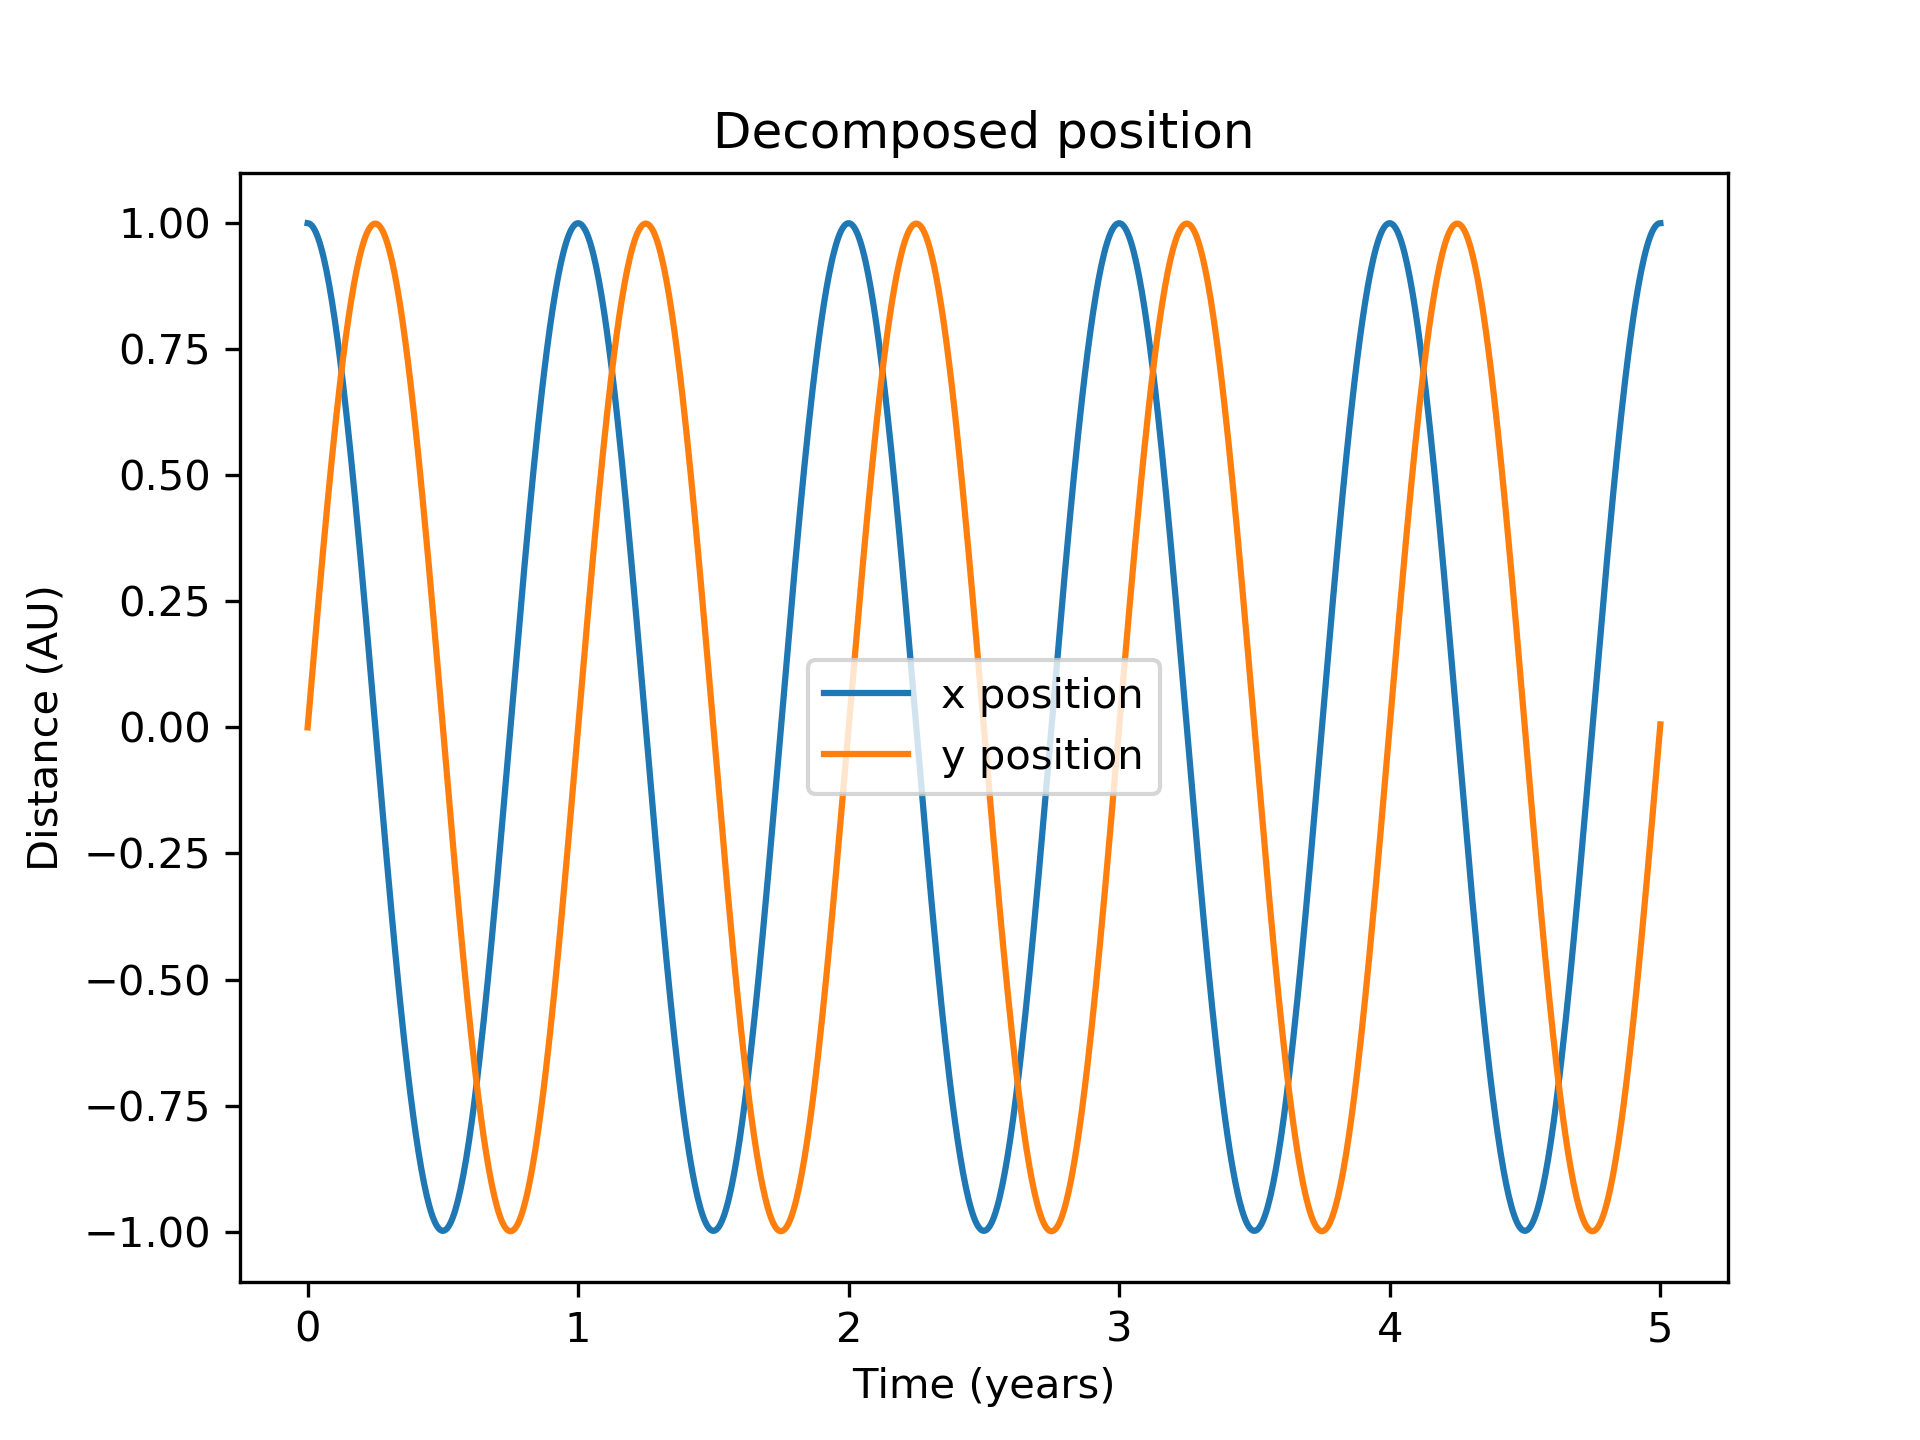
\includegraphics[width=0.8\textwidth]{./Plot/xy_vs_time.png}
            \caption{: x and y position of the Earth relative to the Sun.}
            \label{fig:position}
        \end{center}
    \end{figure}

    \begin{figure}[H]
        \begin{center}
            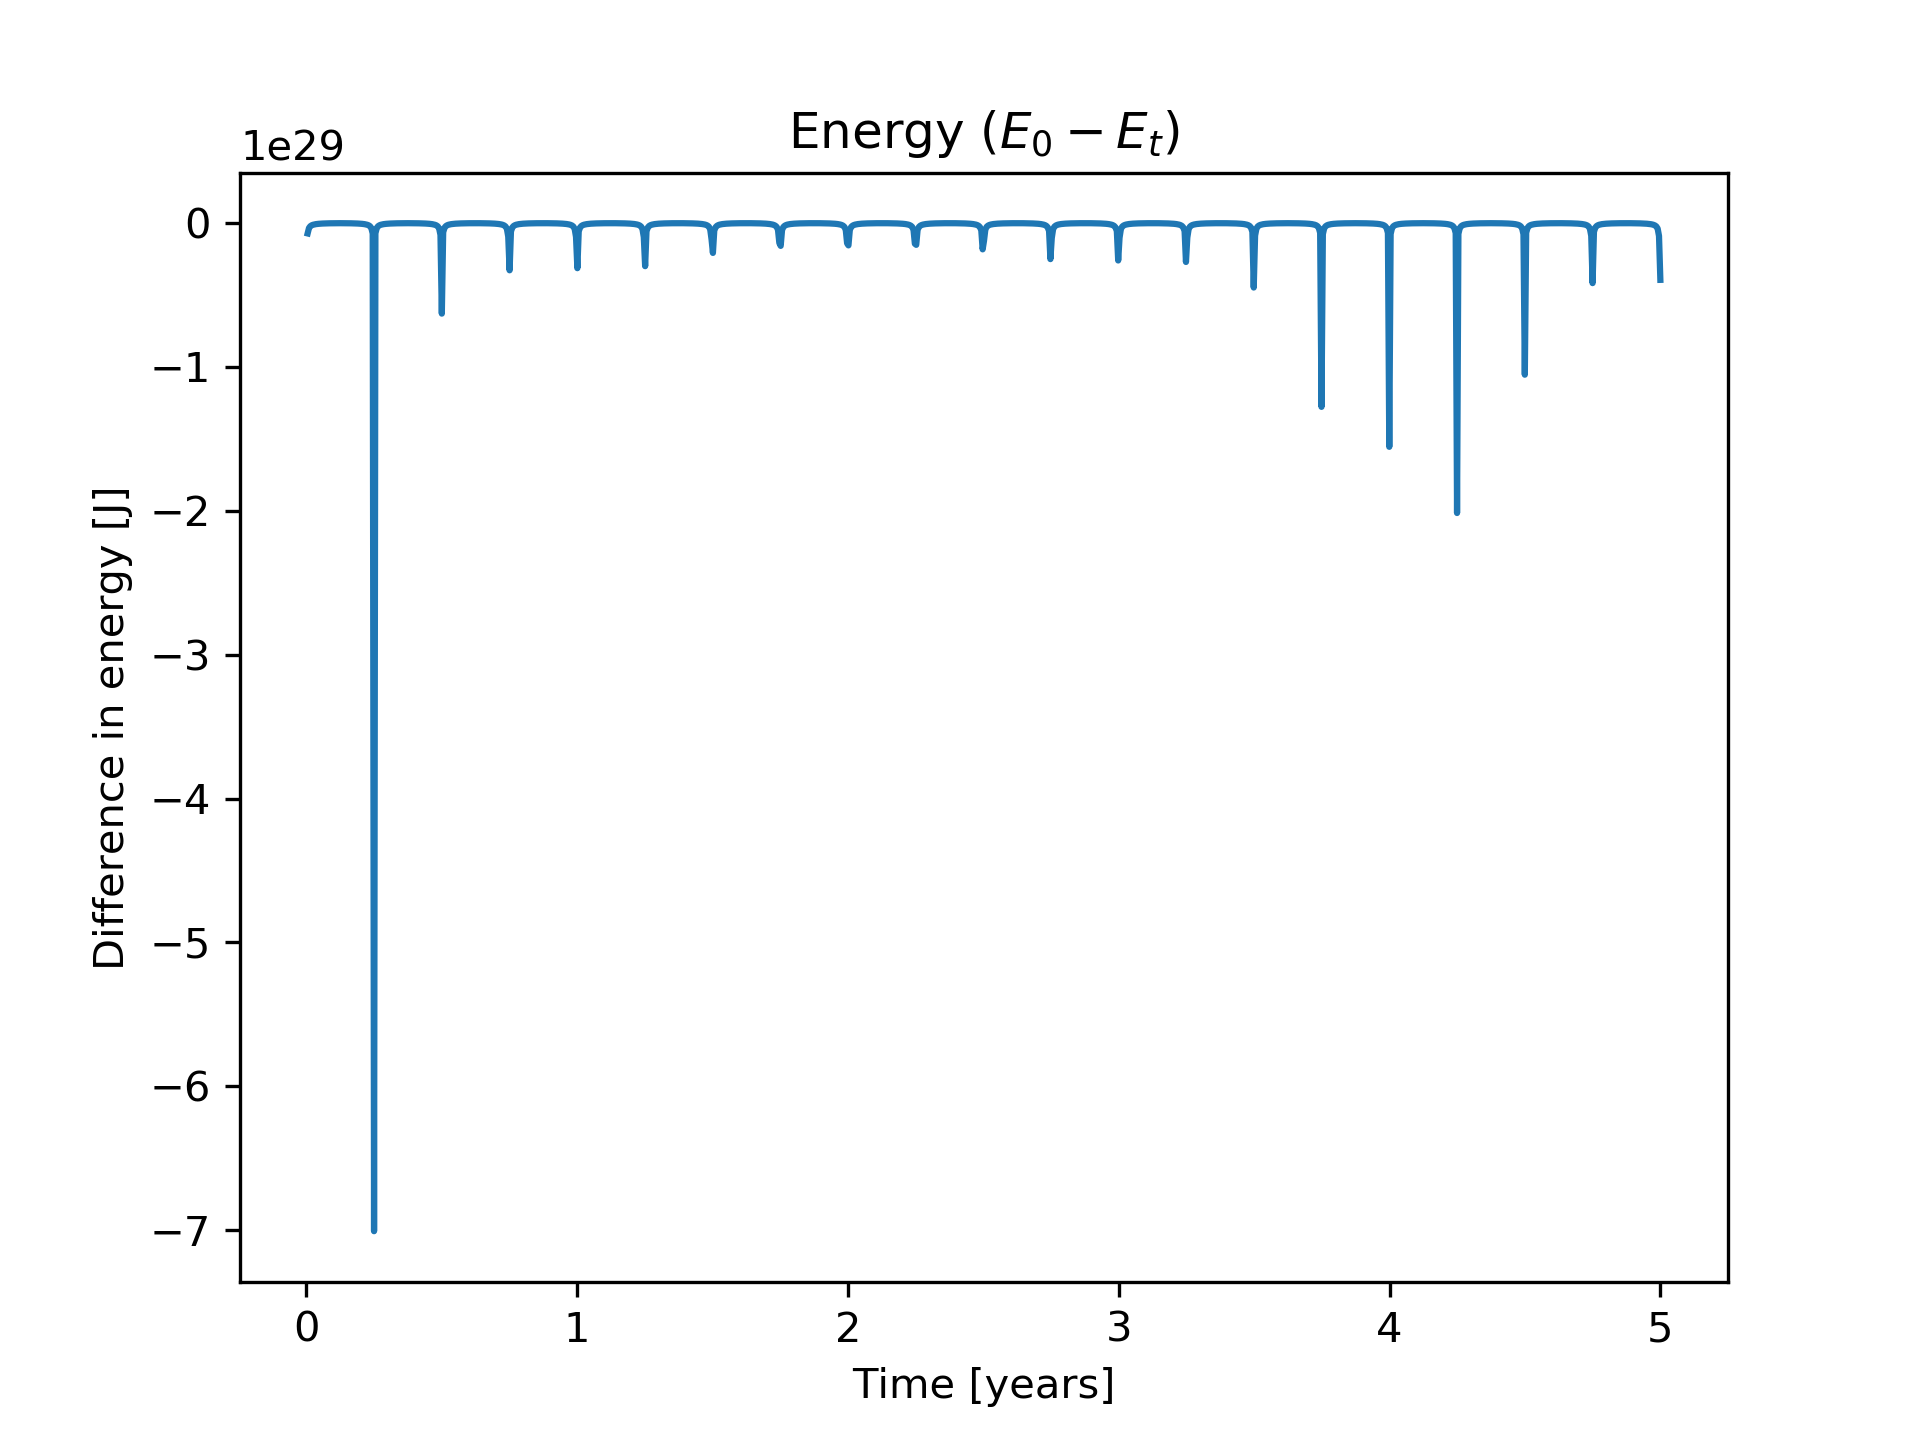
\includegraphics[width=0.8\textwidth]{./Plot/energy.png}
            \caption{: Energy of the Earth plottet against time.
            }
            \label{fig:energy}
        \end{center}
    \end{figure}

    \begin{figure}[H]
        \begin{center}
            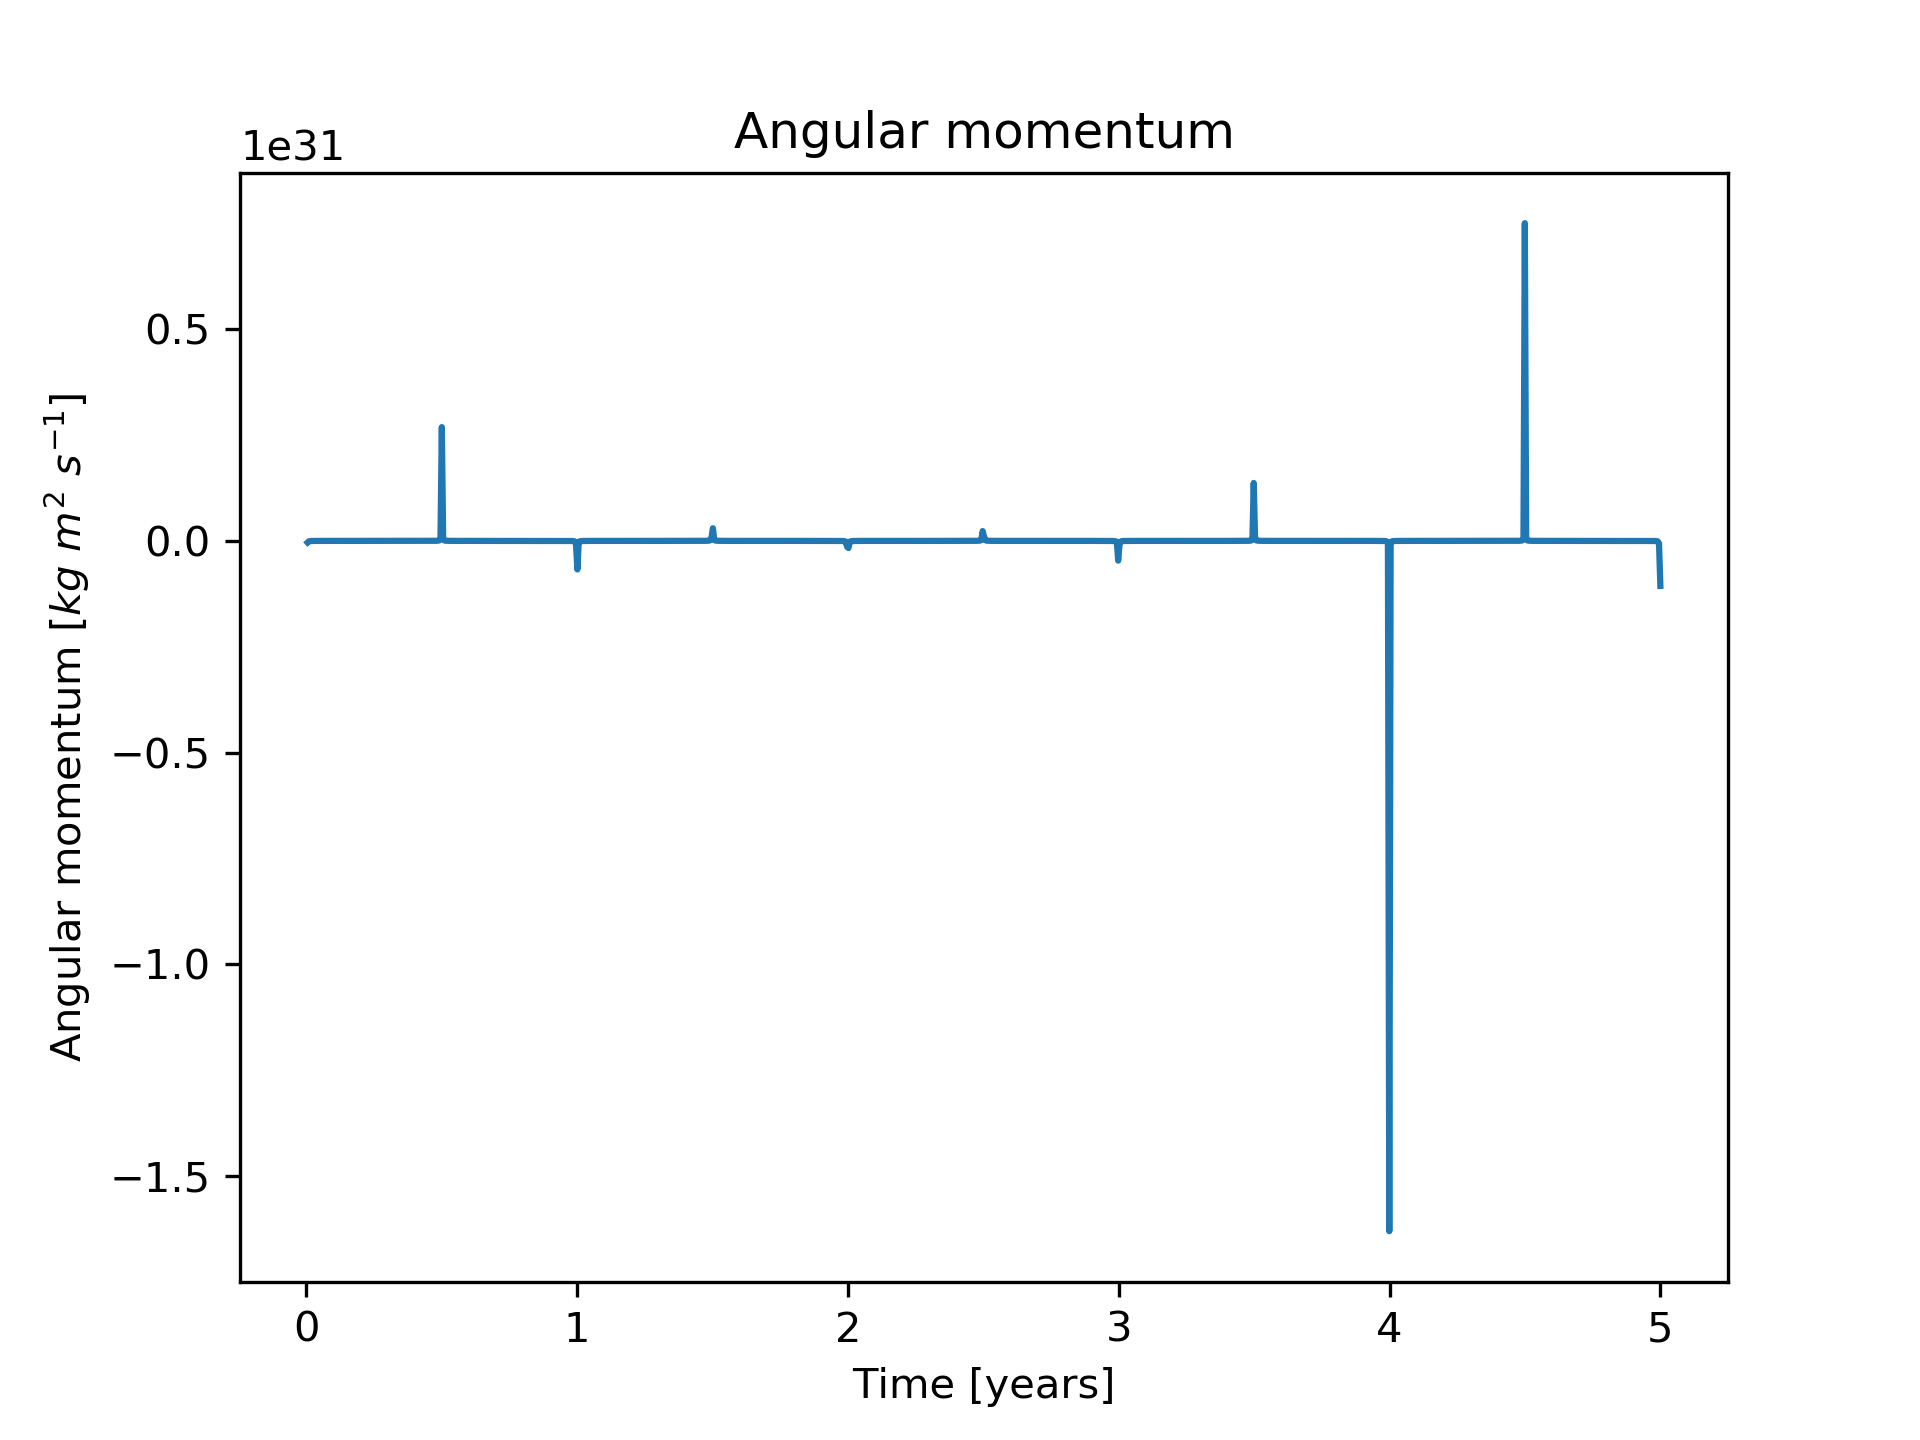
\includegraphics[width=0.8\textwidth]{./Plot/angular_momentum.png}
            \caption{: Angular Momentum}
            \label{fig:am}
        \end{center}
    \end{figure}

    \subsection{Initial velocity for circular orbit}
        We can see from our simulations that the initial velocity needs to be minimum 2$\pi$ AU/(yr) to obtain a circular orbit of the Earth around the Sun.
        The plot of the Earth's orbit around the Sun is shown in Figure \ref{fig:earth_orbit}

        \begin{figure}[H]
            \begin{center}
                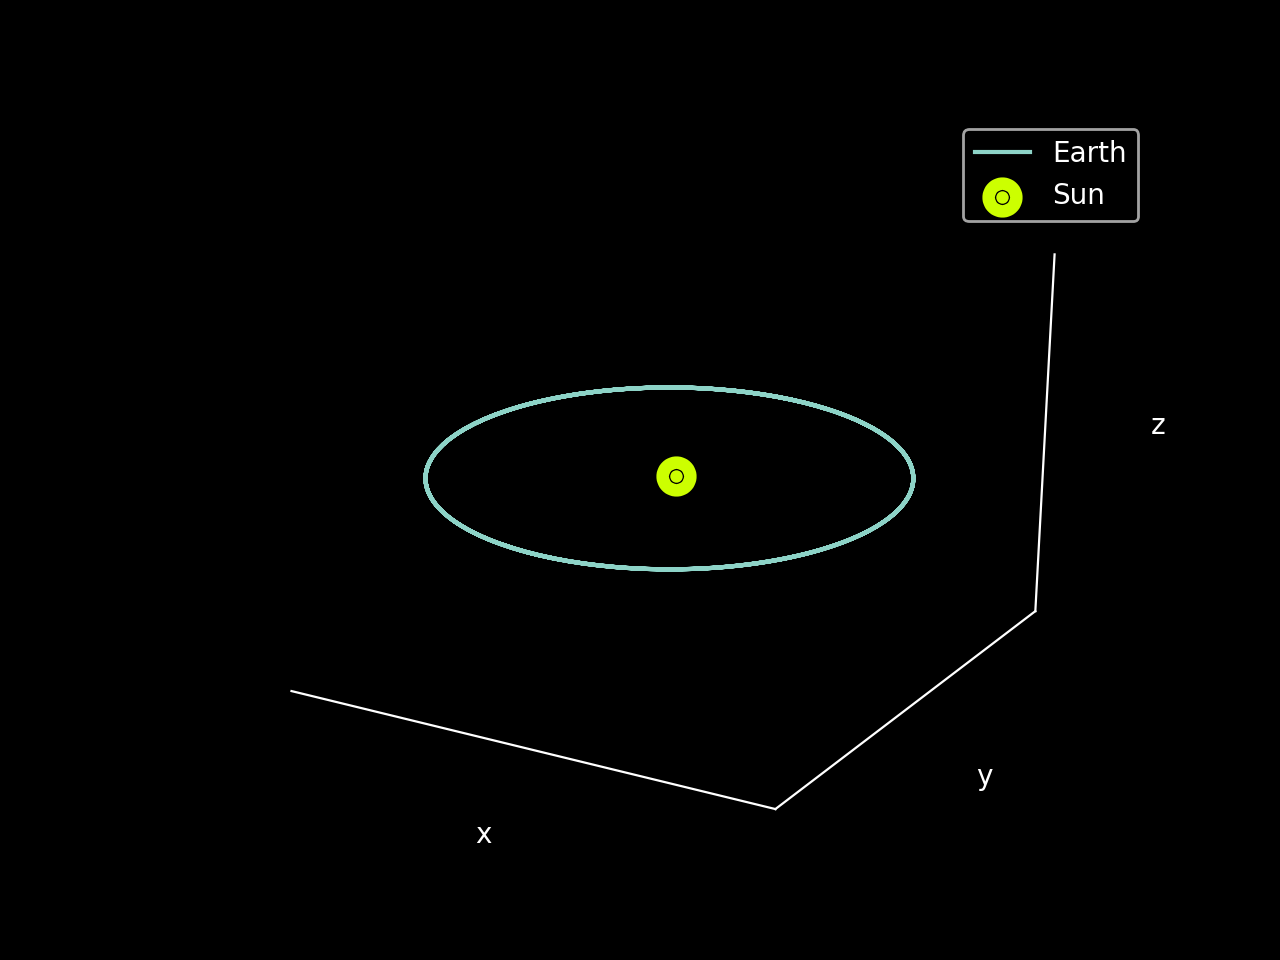
\includegraphics[width=0.8\textwidth]{./Plot/Earth_orbit.png}
                \caption{: Plot of the orbit of the Earth around the Sun.}
                \label{fig:earth_orbit}
            \end{center}
        \end{figure}

    \subsection{Escape velocity}
        When we consider a planet which begins at a distance 1 AU from the Sun, the inital velocity when the planet won't have an orbit at all, but will simply escape from the Sun, is approximately 2.82$\pi$ AU/(yr). At initial velocities over $2\pi$, the planet's orbit is no longer circular. Figure \ref{fig:last} shows the Earth's orbit around the Sun with different initial velocities.

        \begin{figure}[H]
            \makebox[\textwidth]{\makebox[1.5\textwidth]{%
            \begin{subfigure}{.5\textwidth}
                    \centering
                    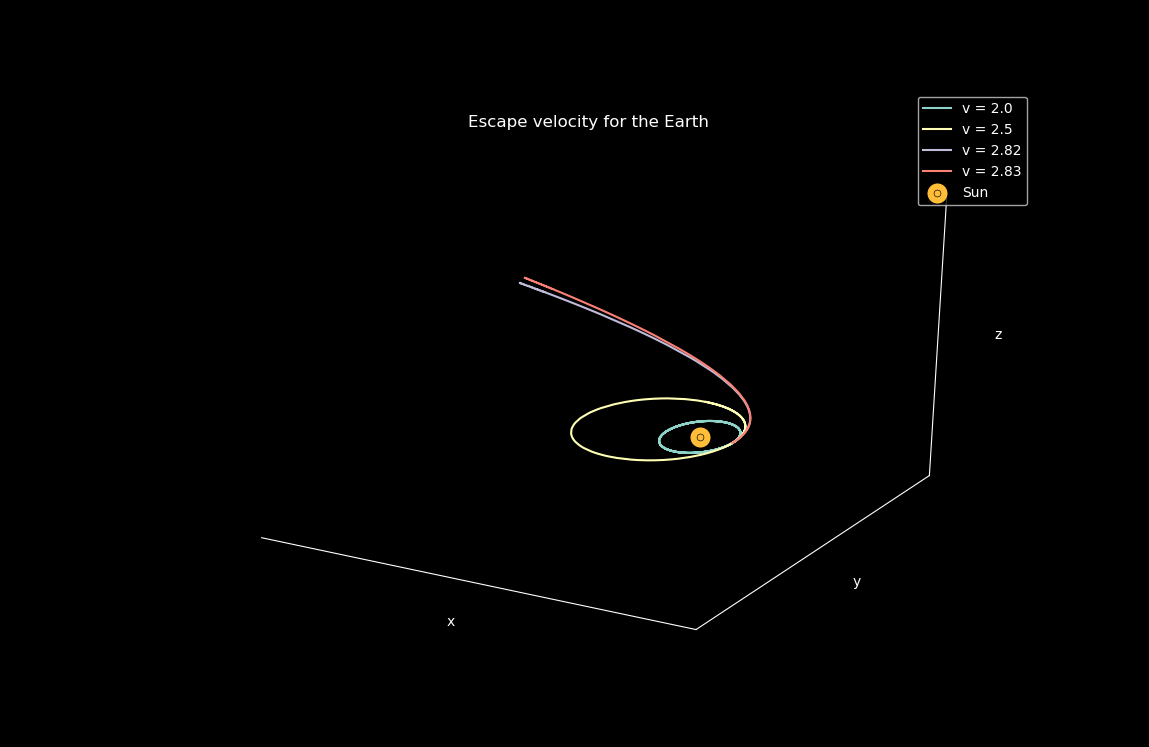
\includegraphics[width=250px]{./Plot/escape_velocity.png}
                    %\caption{}
            \end{subfigure} \hfill %
            \begin{subfigure}{.5\textwidth}
                    \centering
                    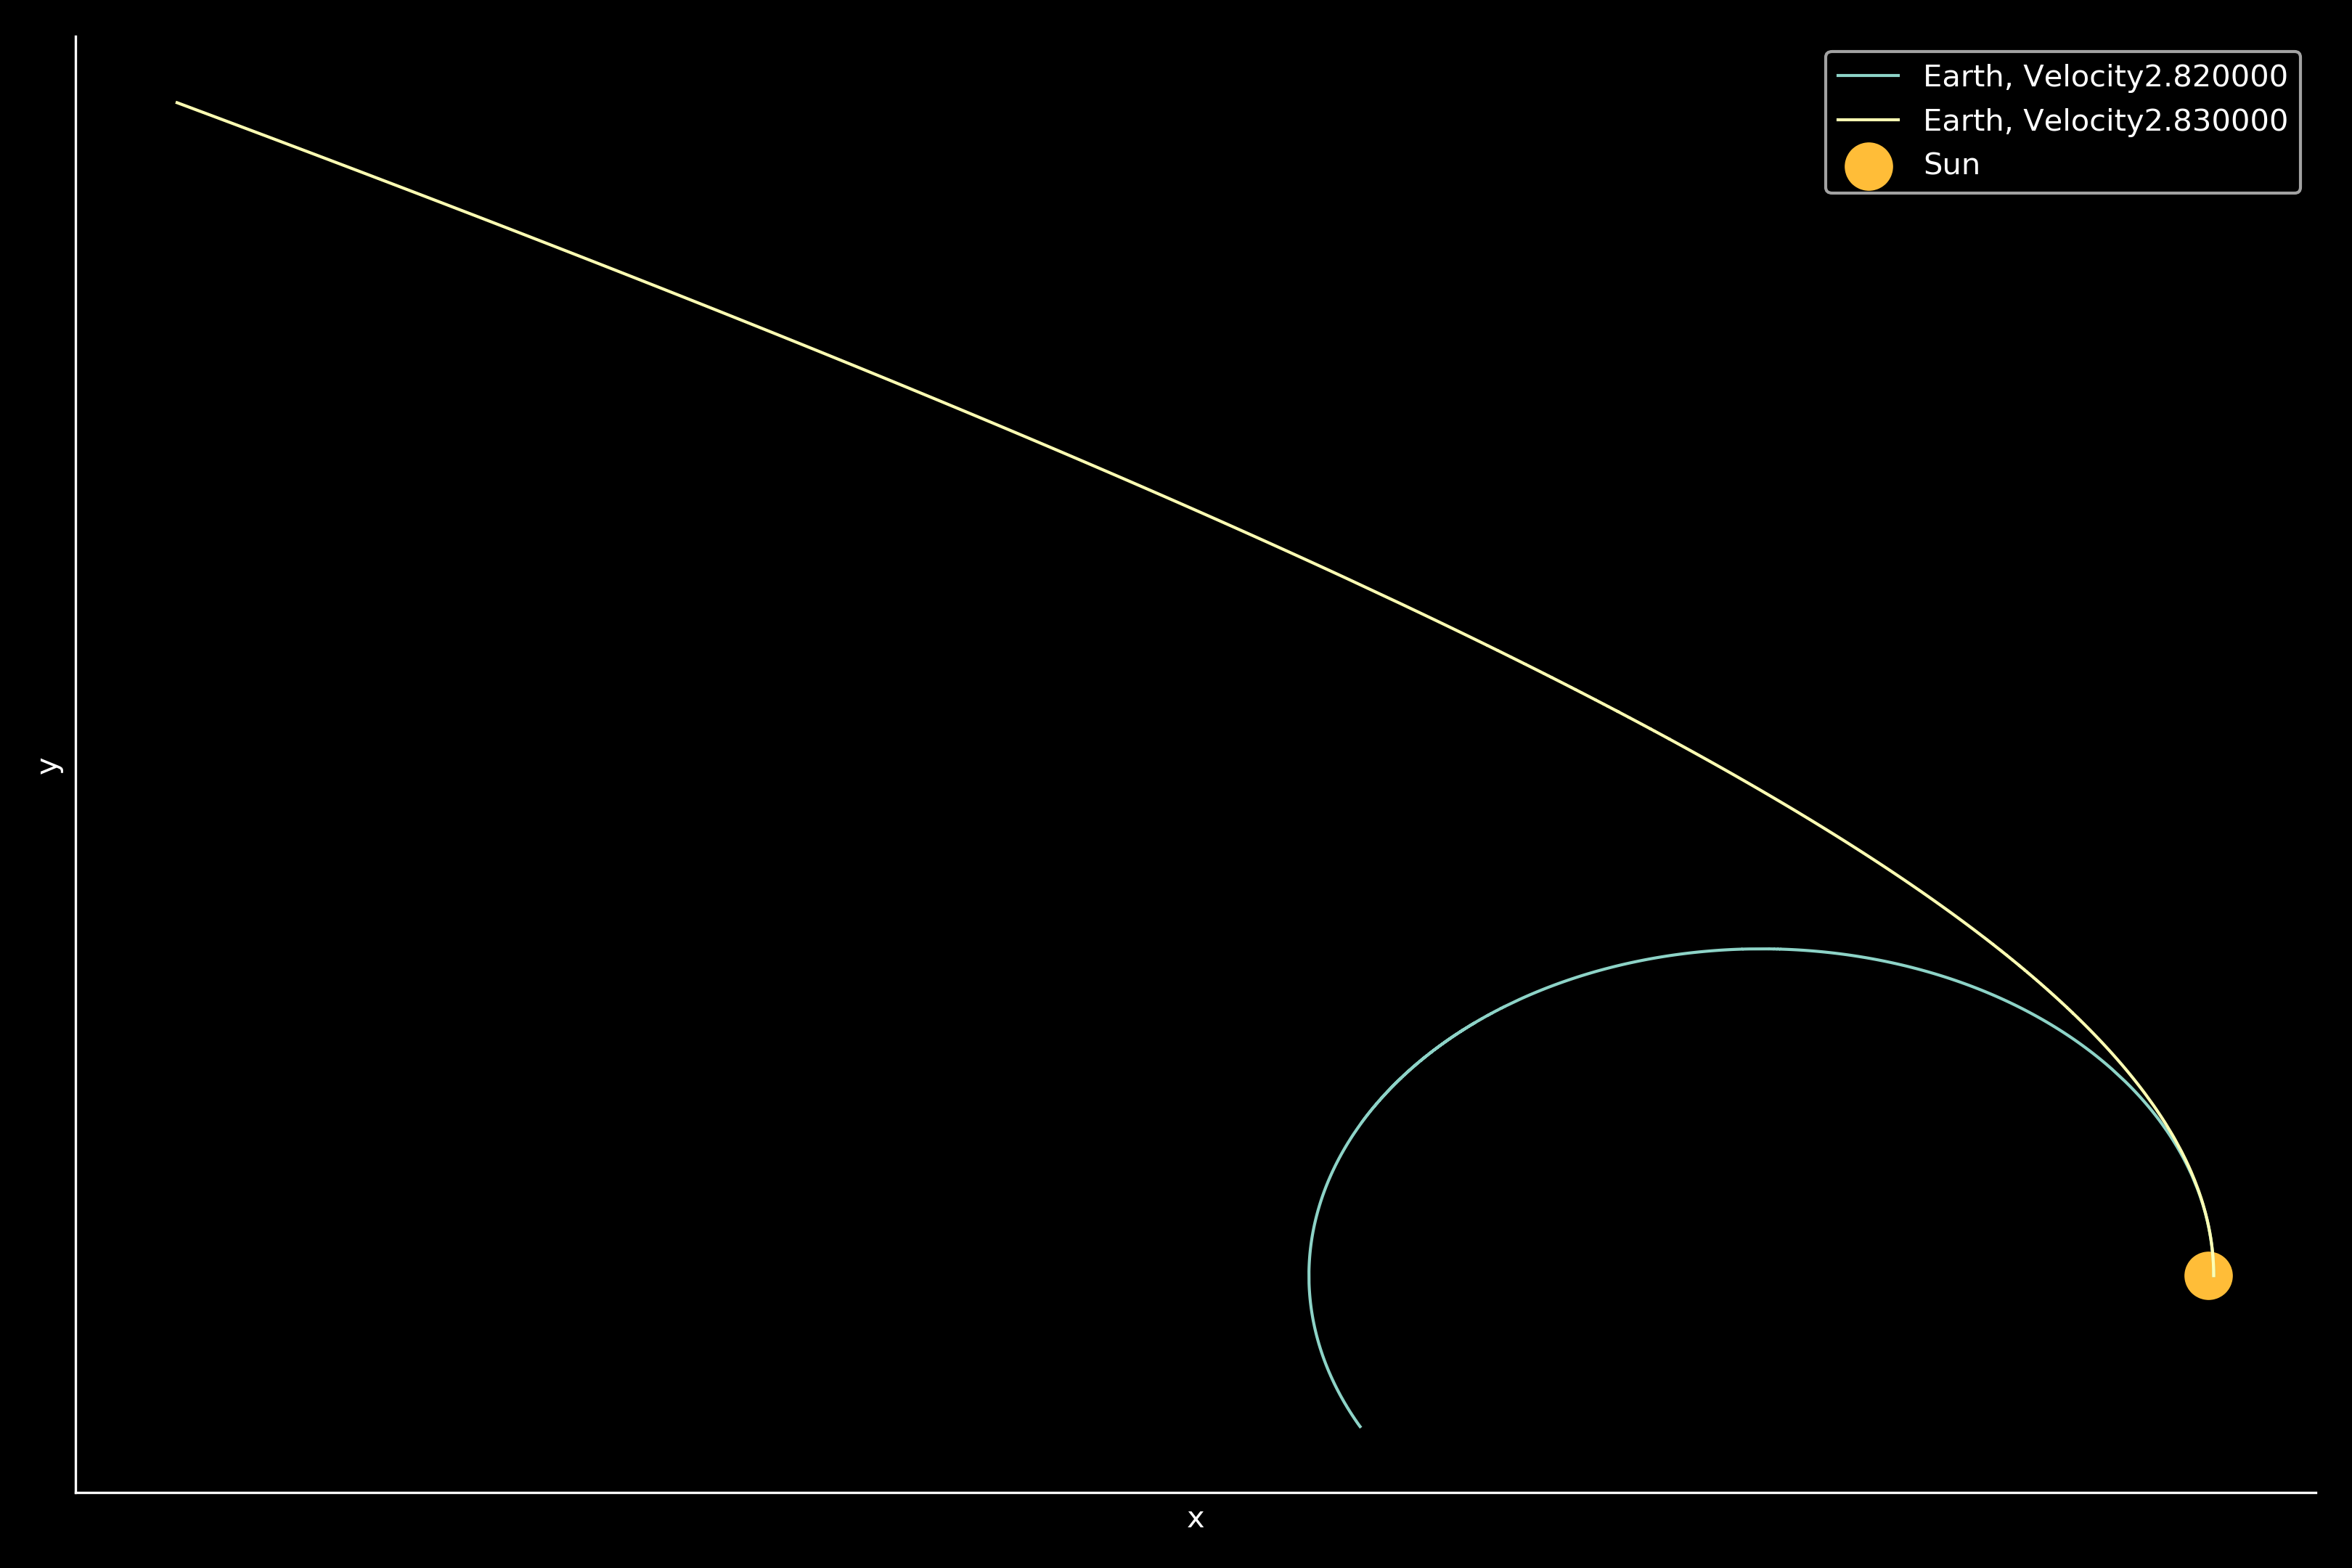
\includegraphics[width=250px]{./Plot/escape_velocity_2.png}
                    %\caption{}
            \end{subfigure}\hfill}}
            \caption{: The Earth-Sun system with different initial velocities.}
            \label{fig:last}
        \end{figure}


    \subsection{Changing the gravitational force}
        If we try to replace the gravitational force from Equation \ref{eq:FG} with

        \begin{flalign}
            F_G = \frac{GM_{\odot}M_E}{r^{\beta}}
            \label{eq:beta}
        \end{flalign}

        with $\beta \in [2,3]$, we effectively modify the force of gravity. The results of this experiment is shown in Figure \ref{fig:beta}. These figures shows that when $\beta$ approches 3, the Earth begins to escape the sun.

        \begin{figure}[H]
            \makebox[\textwidth]{\makebox[1.5\textwidth]{%
            \begin{subfigure}{.5\textwidth}
                    \centering
                    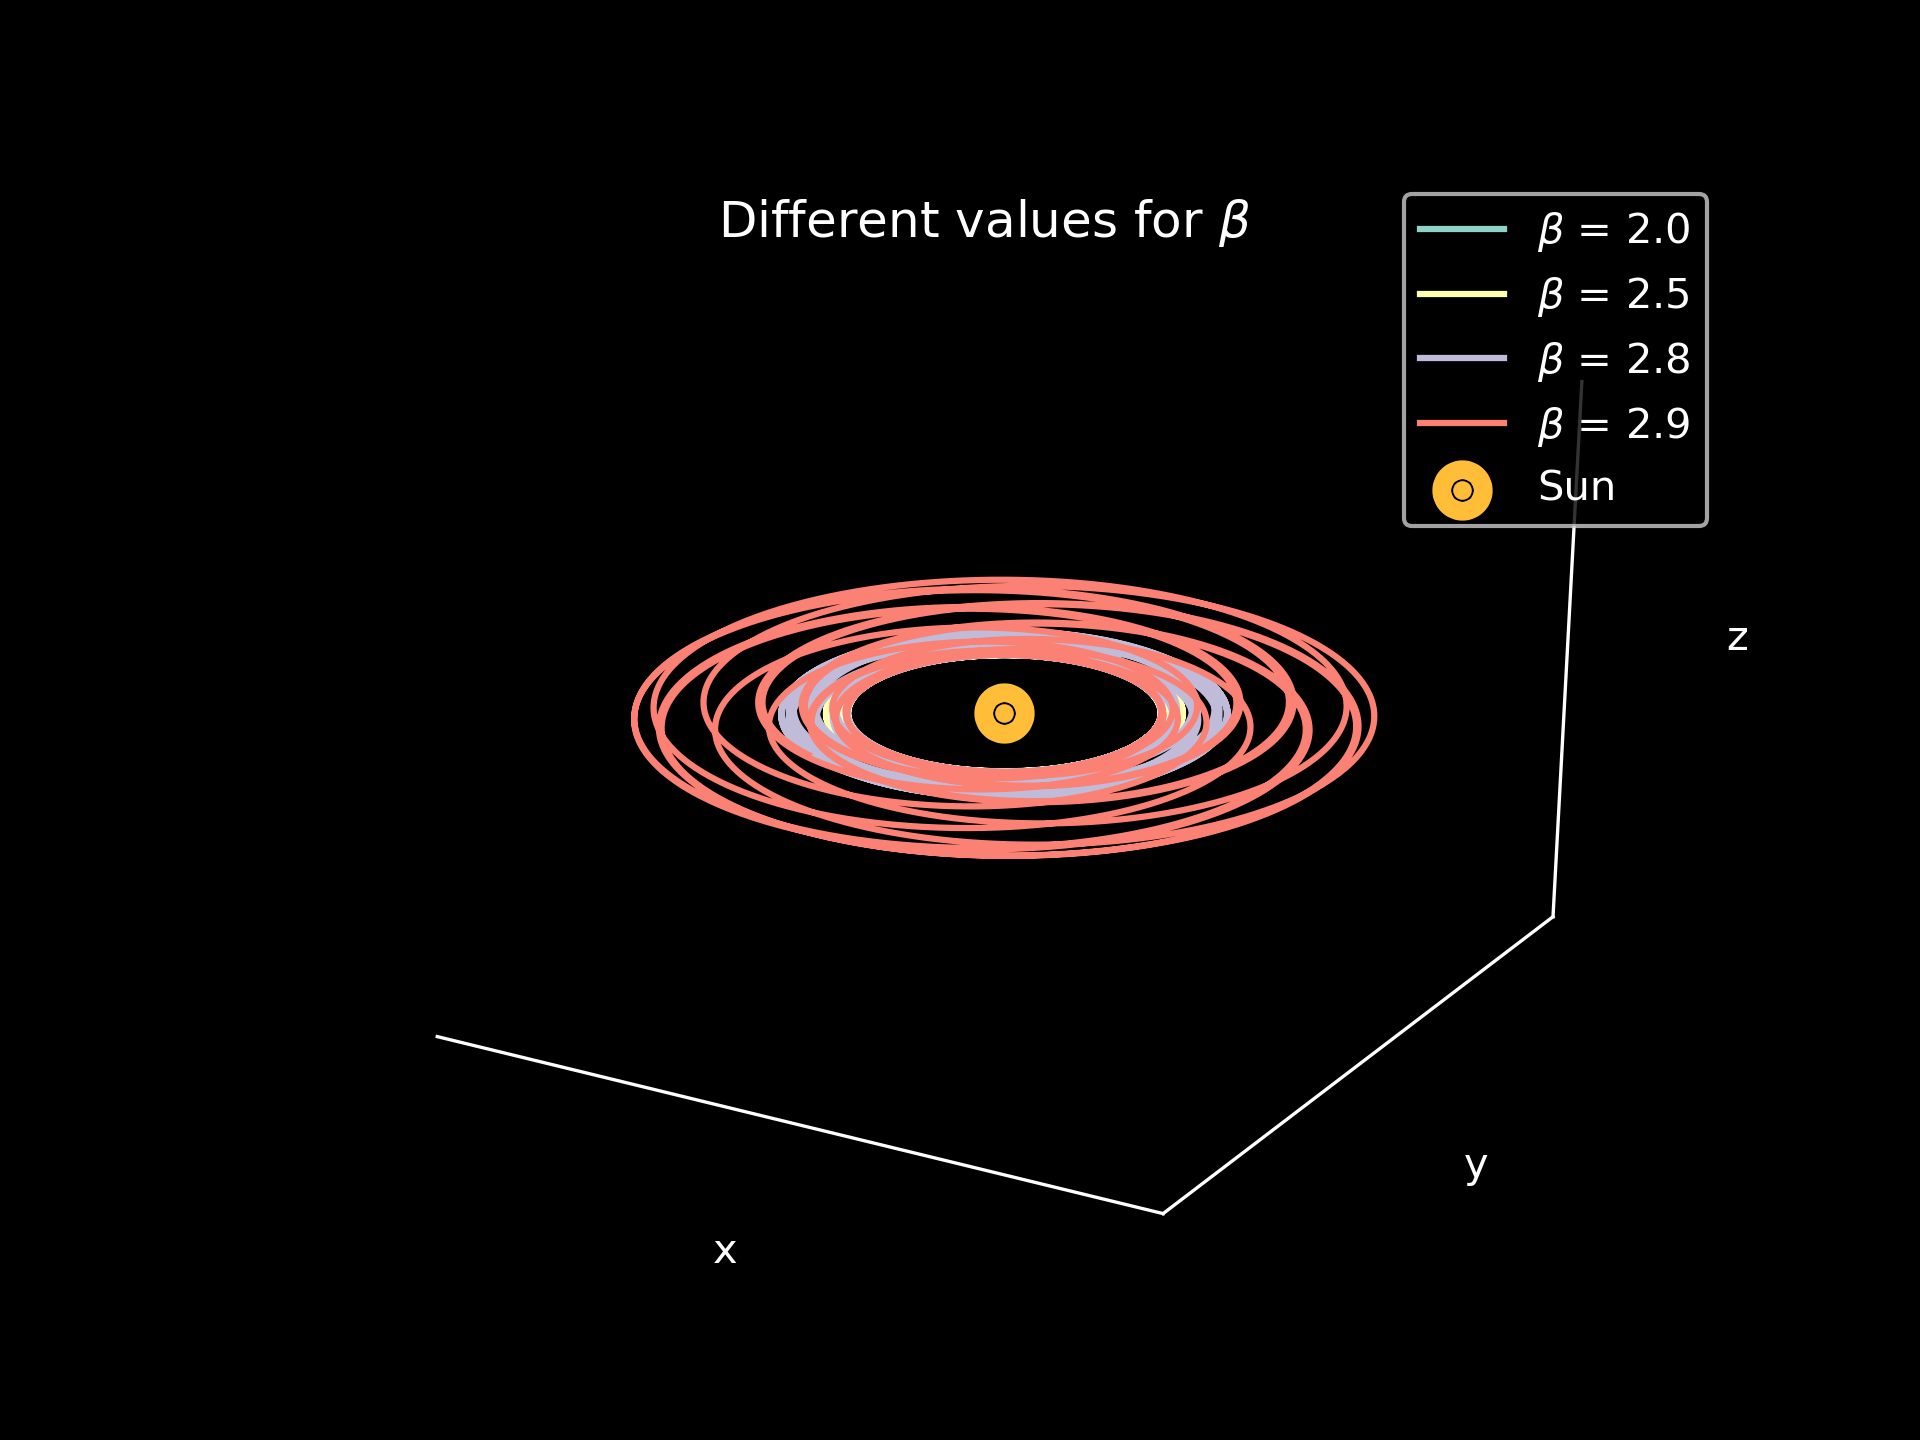
\includegraphics[width=250px]{./Plot/vary_beta_1.png}
                    %\caption{}
            \end{subfigure} \hfill %
            \begin{subfigure}{.5\textwidth}
                    \centering
                    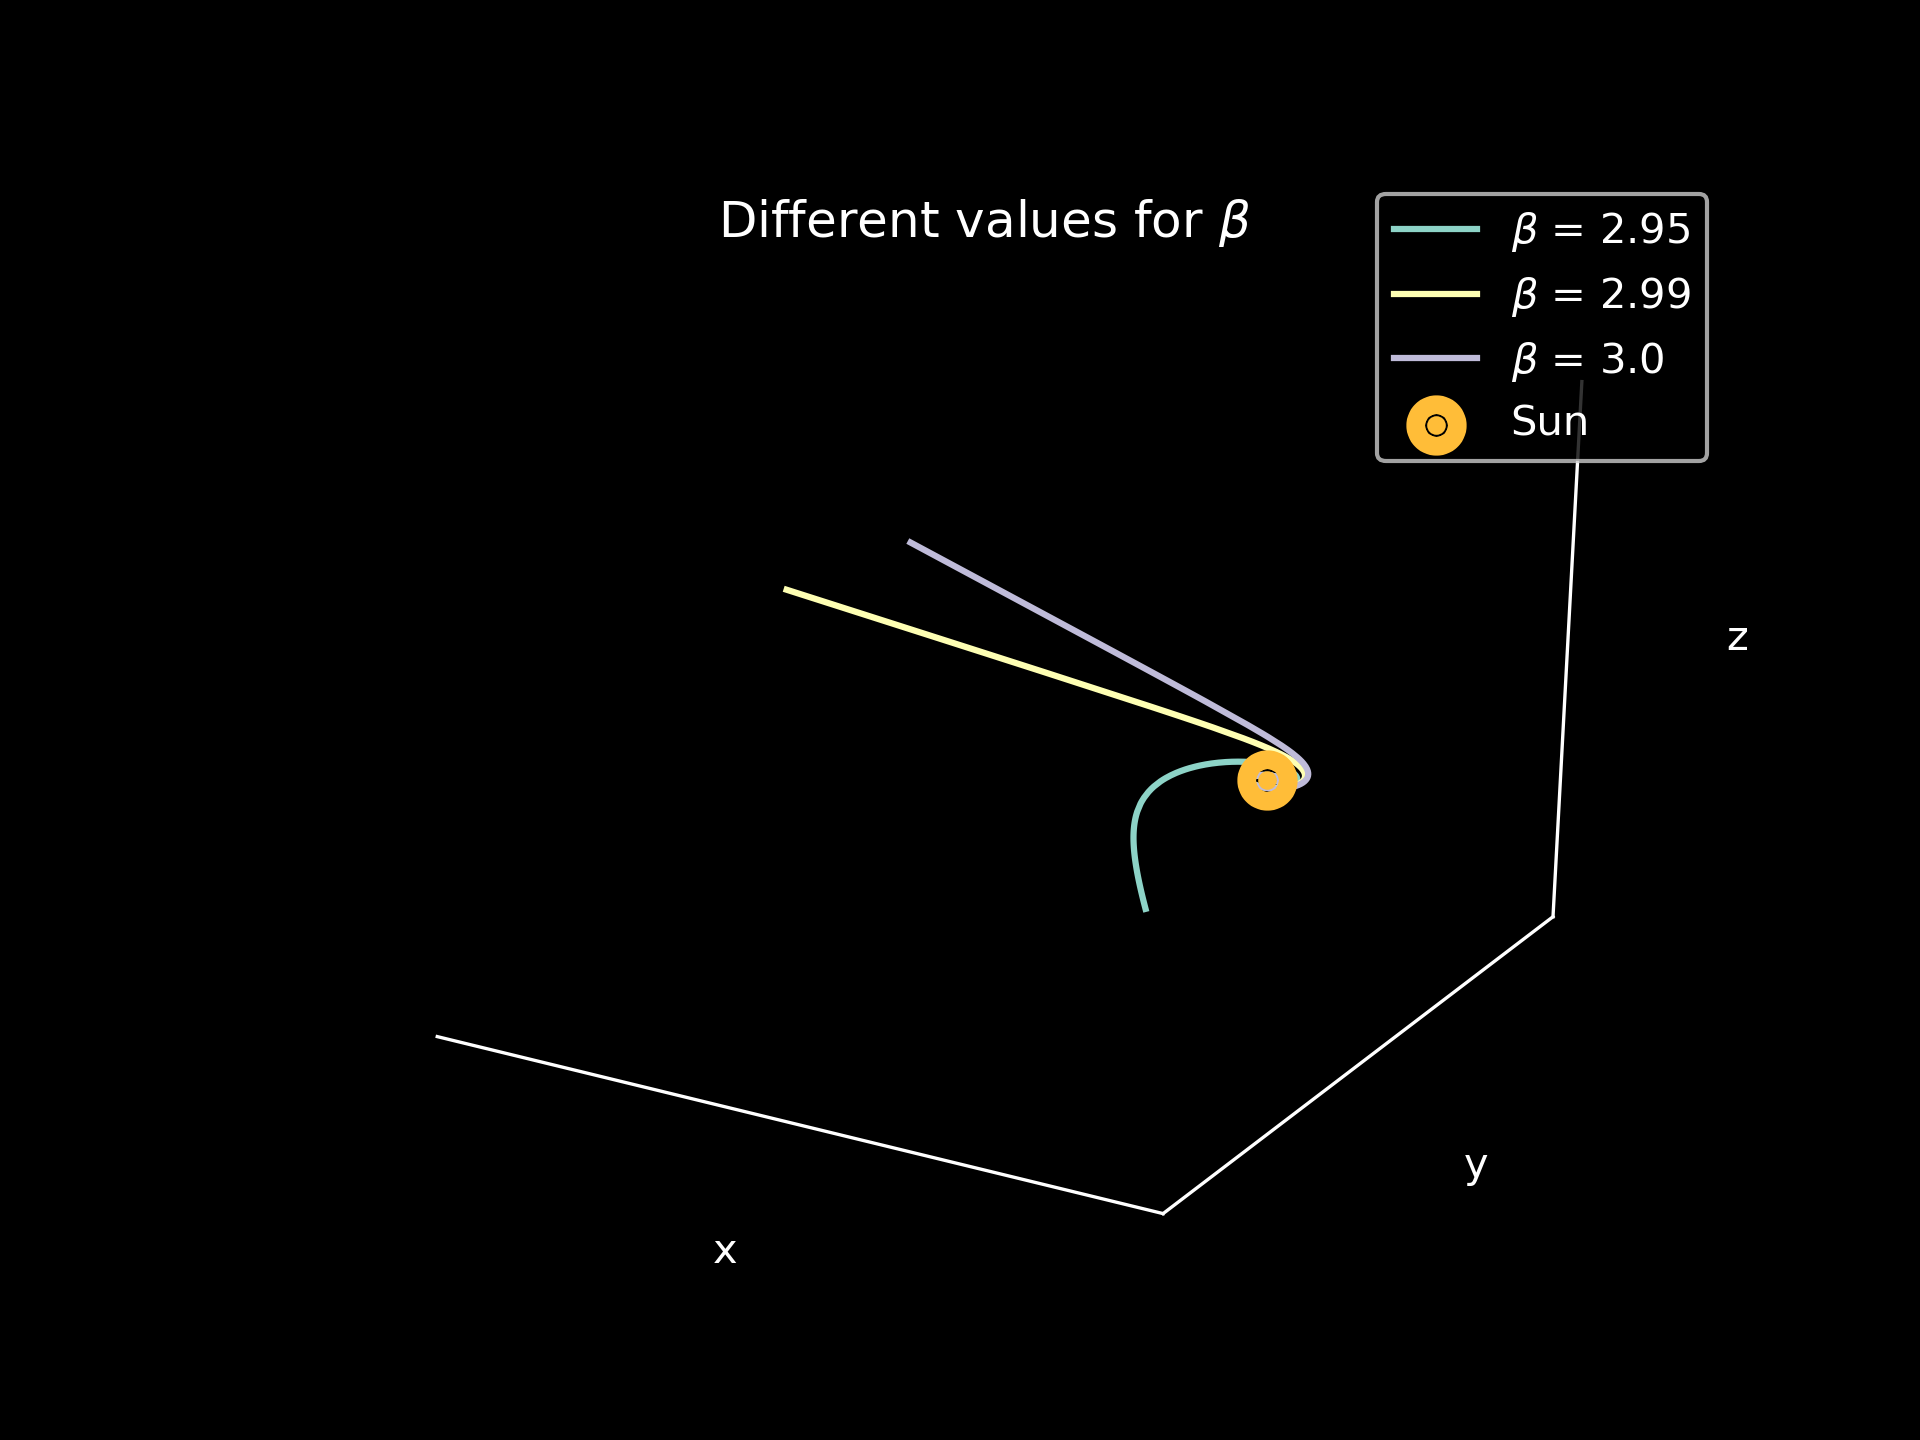
\includegraphics[width=250px]{./Plot/vary_beta_2.png}
                    %\caption{}
            \end{subfigure}\hfill}}
            \caption{: The Earth-Sun system for different values of $\beta$.}
            \label{fig:beta}
        \end{figure}

    \subsection{Adding Jupiter to the system}
        We then add Jupiter to our system. We evaluate how Jupiter affects the orbit of the Earth when we increase Jupiters mass. The result when Jupiter has it's real mass is shown in Figure \ref{fig:jupiter1}. When we increase the mass with a factor of 10, the result does not differ from what we see in Figure \ref{fig:jupiter1}. Figure \ref{fig:jupiter} shows what will happen when we increase the mass of Jupiter with a factor of respectively 950 and 1000. These figures show that when the mass of Jupiter increases it will attract the Earth away from its normal orbit around the Sun. When we increase the mass with a factor of 1000, the Earth will escape both the Sun and Jupiter, because the attraction on Earth from Jupiter is so large, the speed the Earth gains is too high, which propels the Earth away. When Jupiter's mass is increased with a factor of 950, we needed about 20 000 steps for the system to be stable for 20 years.

        \begin{figure}[H]
            \begin{center}
                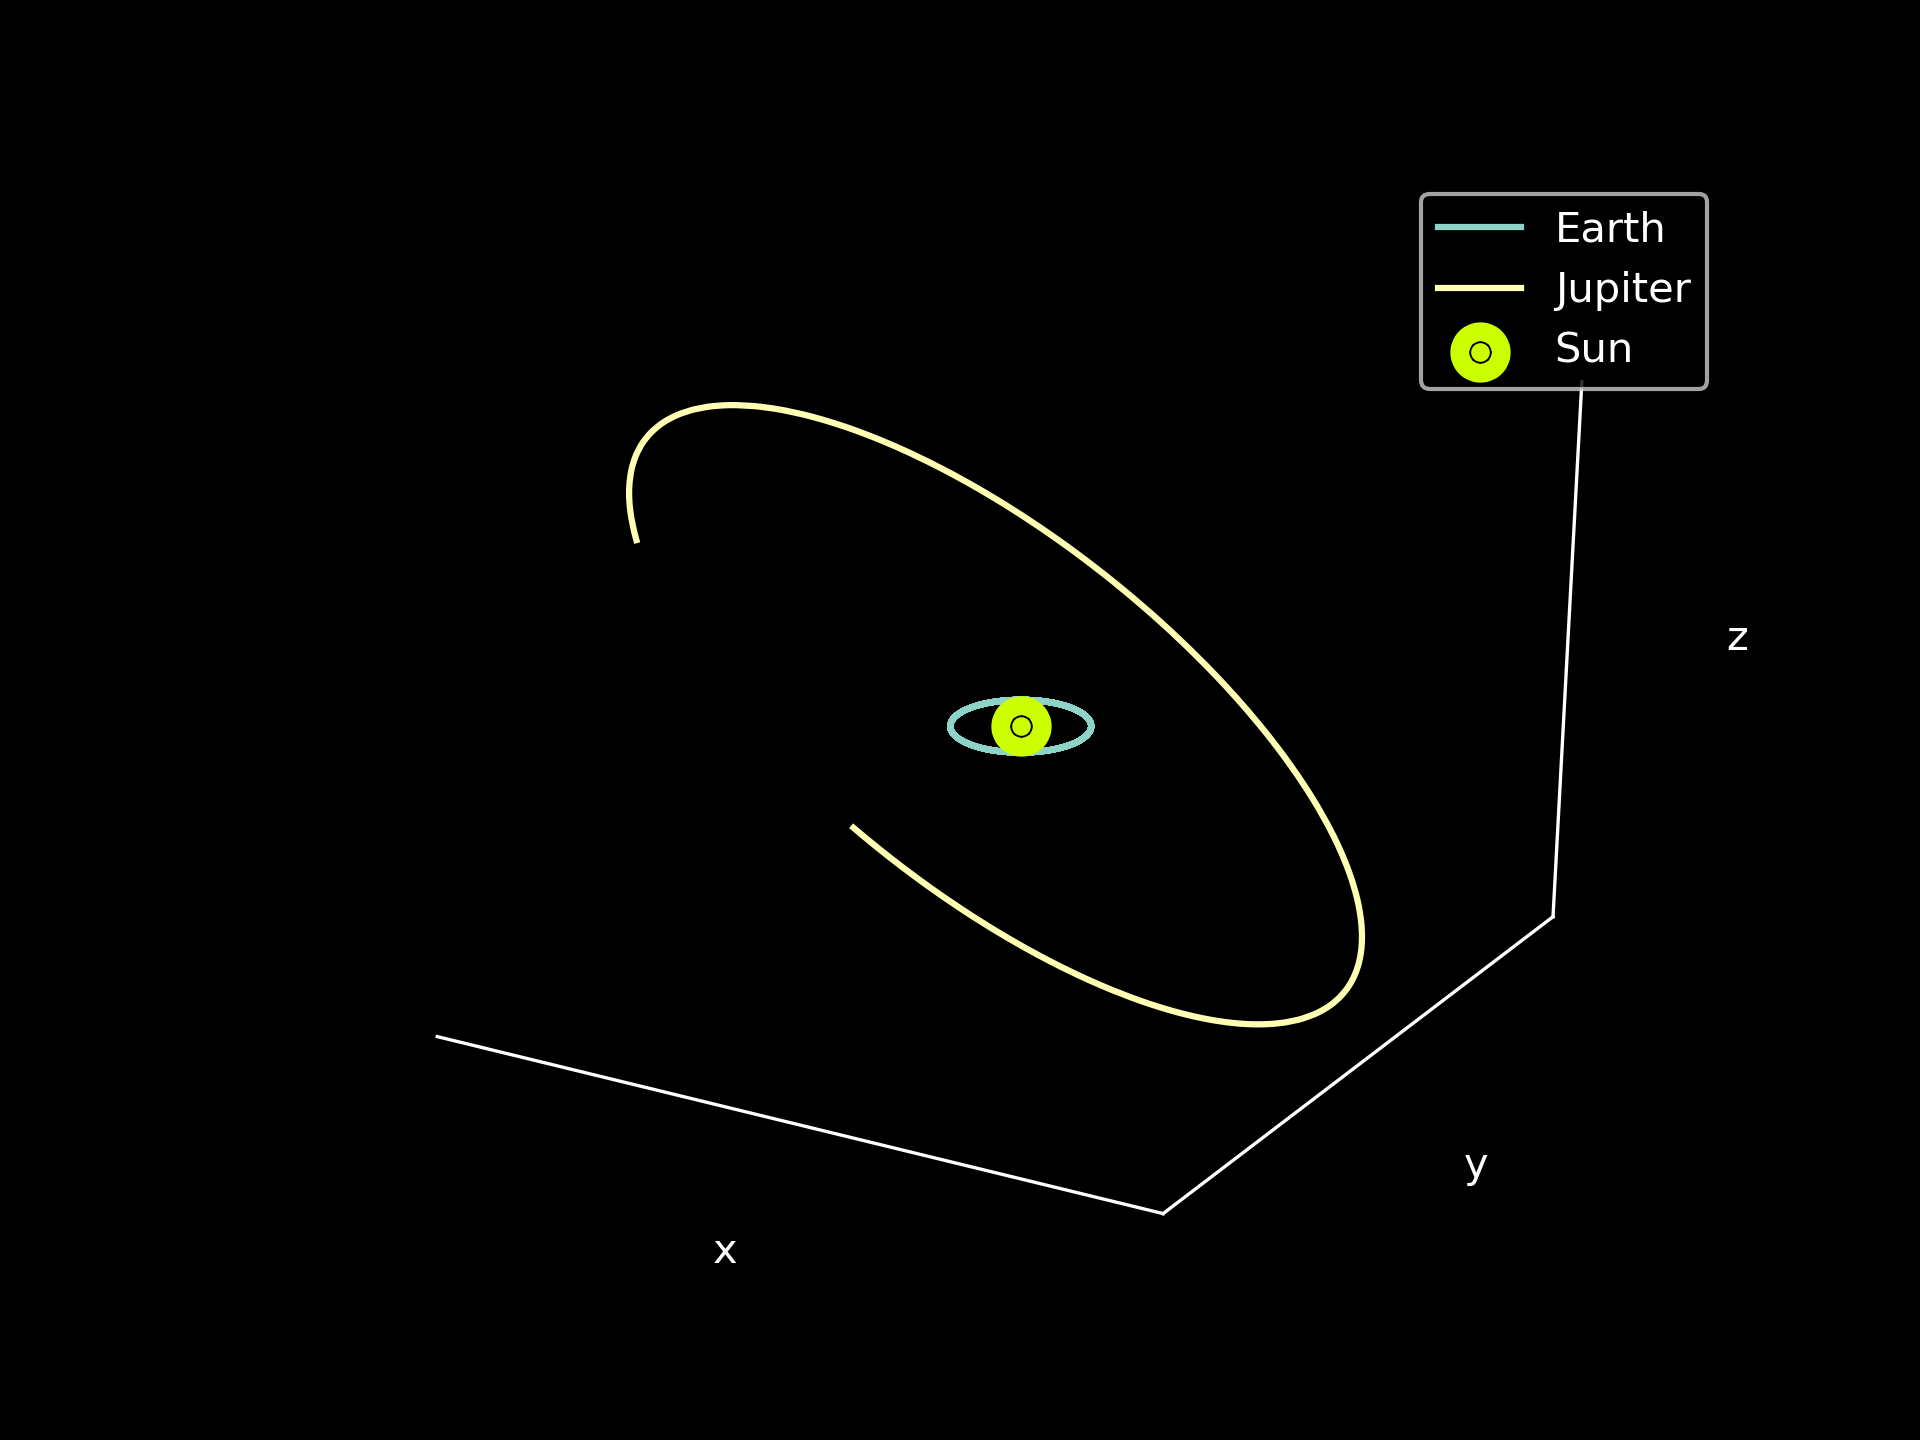
\includegraphics[width=0.8\textwidth]{./Plot/Earth_Jupiter1.png}
                \caption{: Solar system including Earth and Jupiter.}
                \label{fig:jupiter1}
            \end{center}
        \end{figure}

        \begin{figure}[H]
            \makebox[\textwidth]{\makebox[1.5\textwidth]{%
            \begin{subfigure}{.5\textwidth}
                    \centering
                    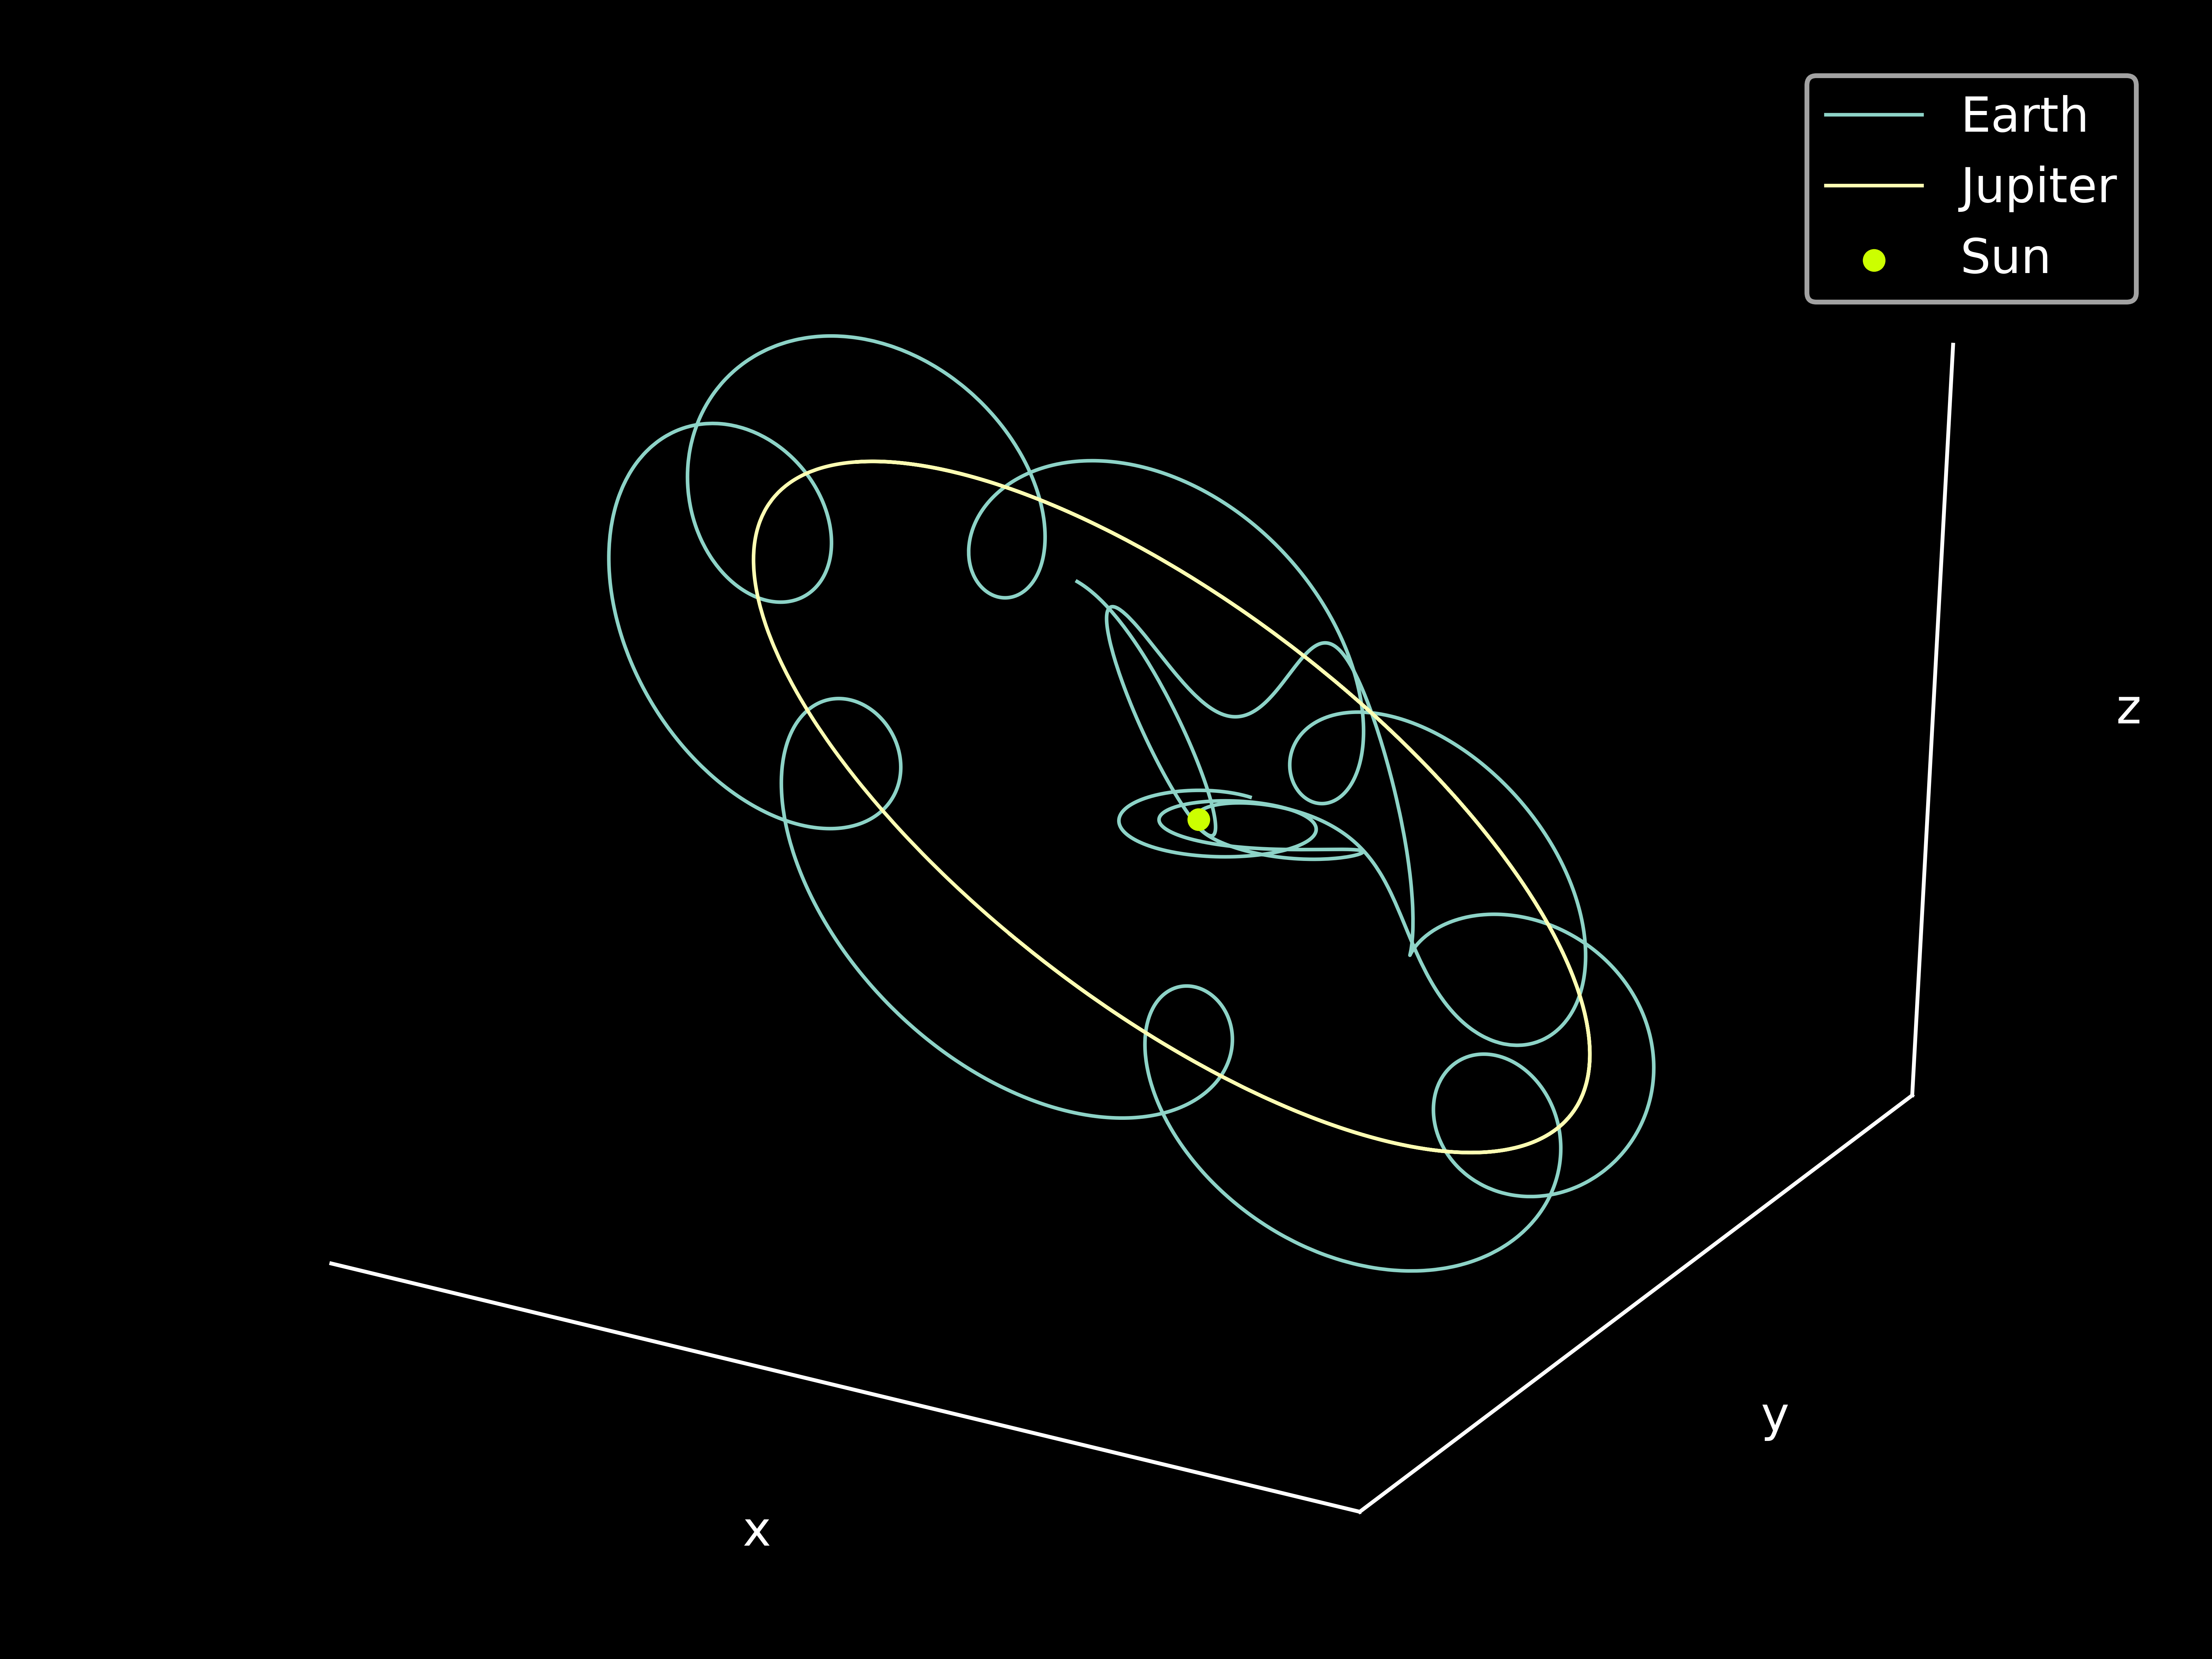
\includegraphics[width=250px]{./Plot/950.png}
                    \caption{Mass of Jupiter increased with a factor of 950}
            \end{subfigure} \hfill %
            \begin{subfigure}{.5\textwidth}
                    \centering
                    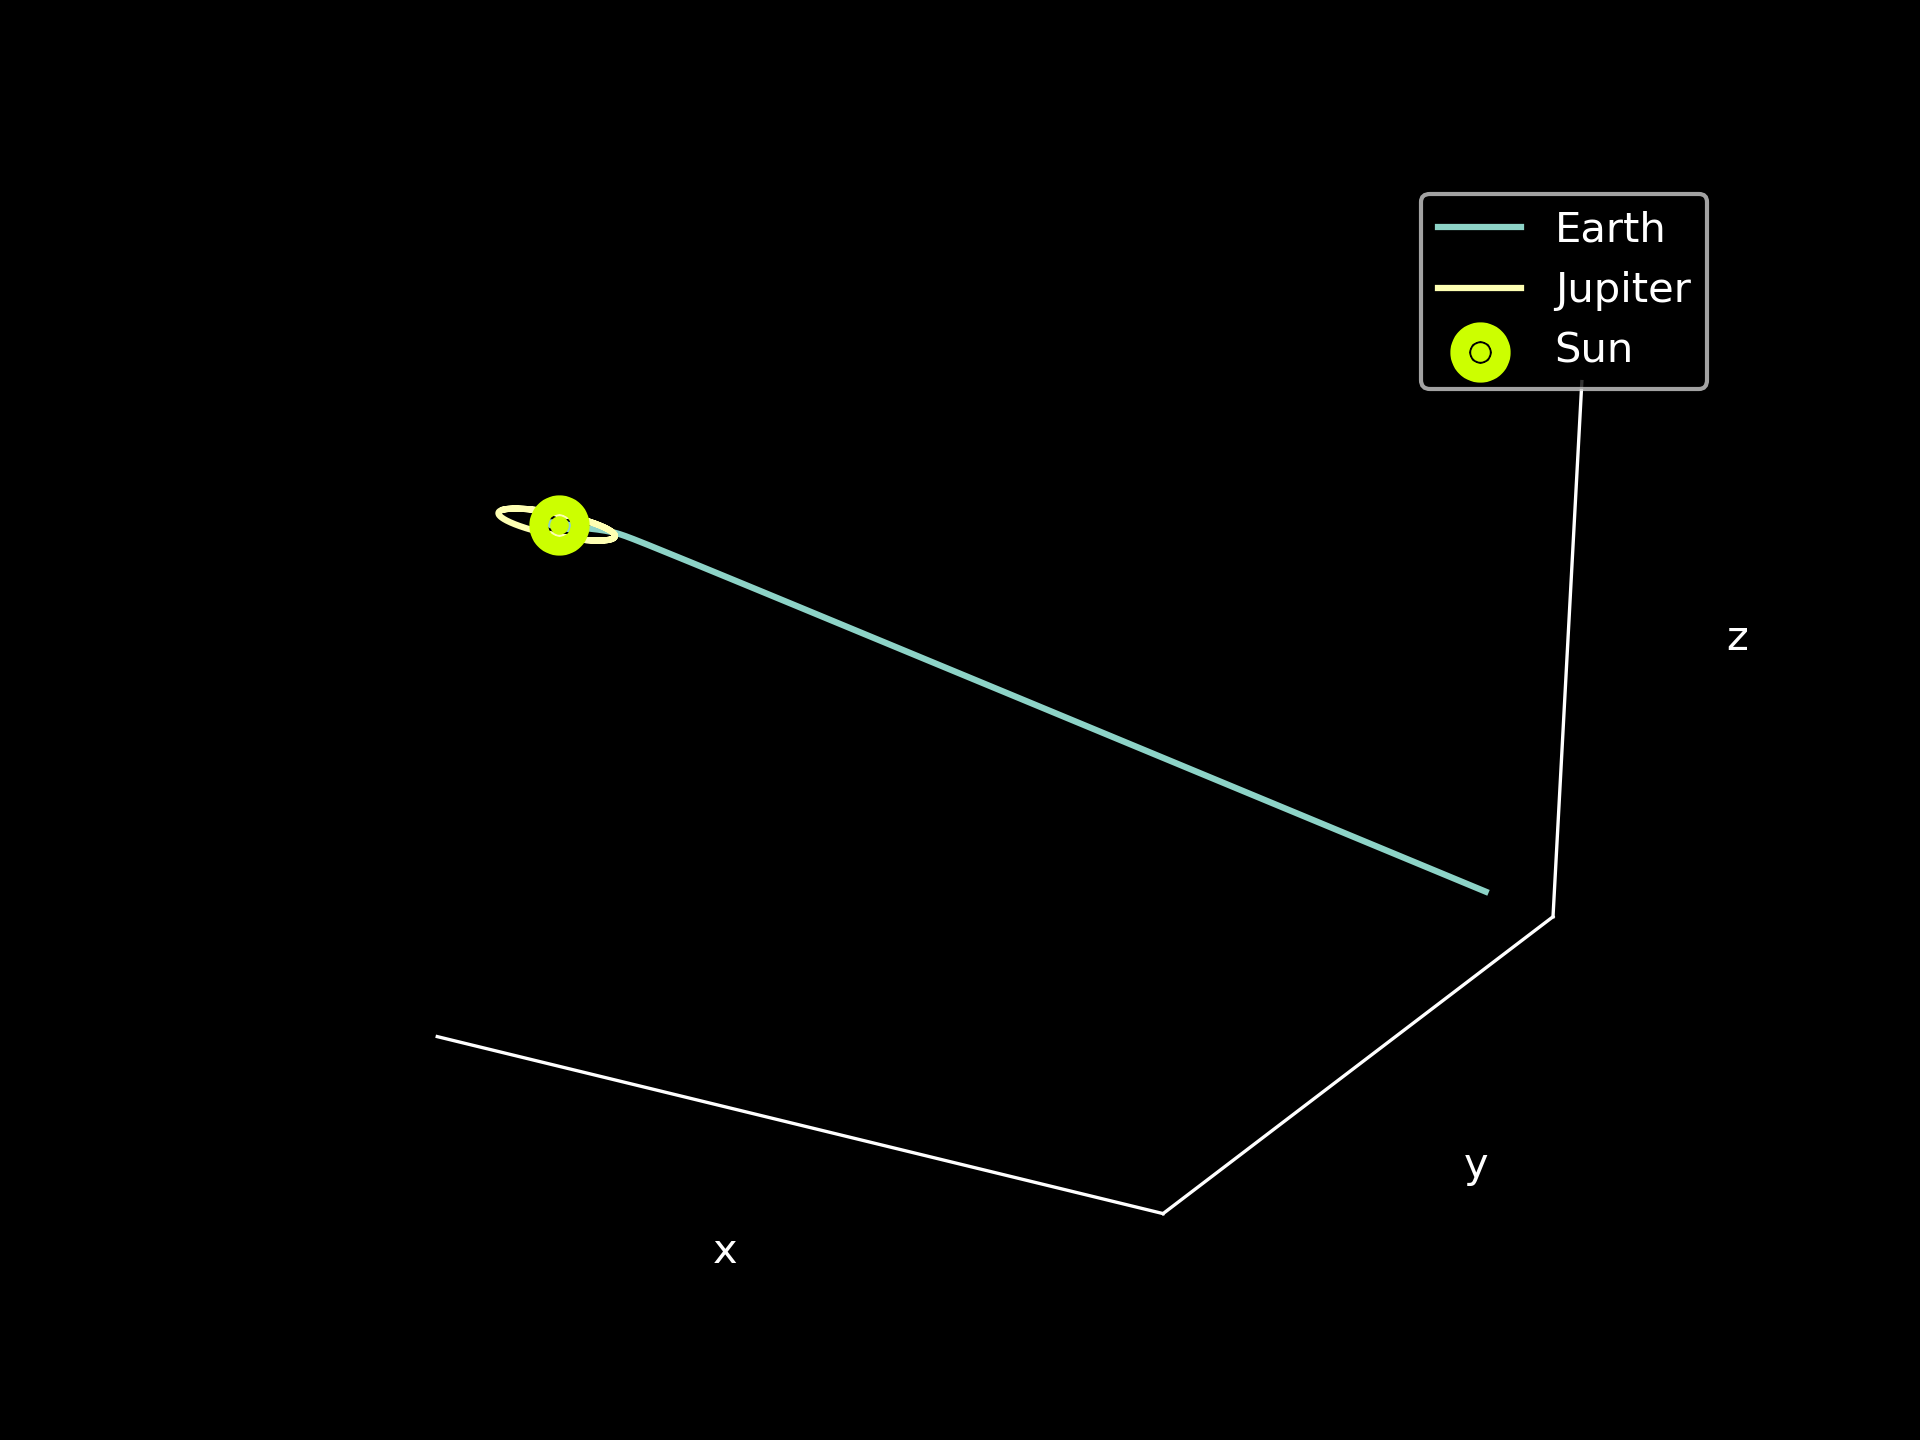
\includegraphics[width=250px]{./Plot/Earth_Jupiter1000.png}
                    \caption{Mass off Jupiter increased with a factor of 1000}
            \end{subfigure}\hfill}}
            \caption{: Solar system including Earth and Jupiter, with the mass of Jupiter increased.}
            \label{fig:jupiter}
            \end{figure}

        \subsection{Finished solar system}
            Further, we have simulated the whole solar system by adding the remaining planets. We have plotted the system with 500 000 integration points over 164 years. The results is represented in Figure \ref{fig:solar}.

            \begin{figure}[H]
                \begin{center}
                    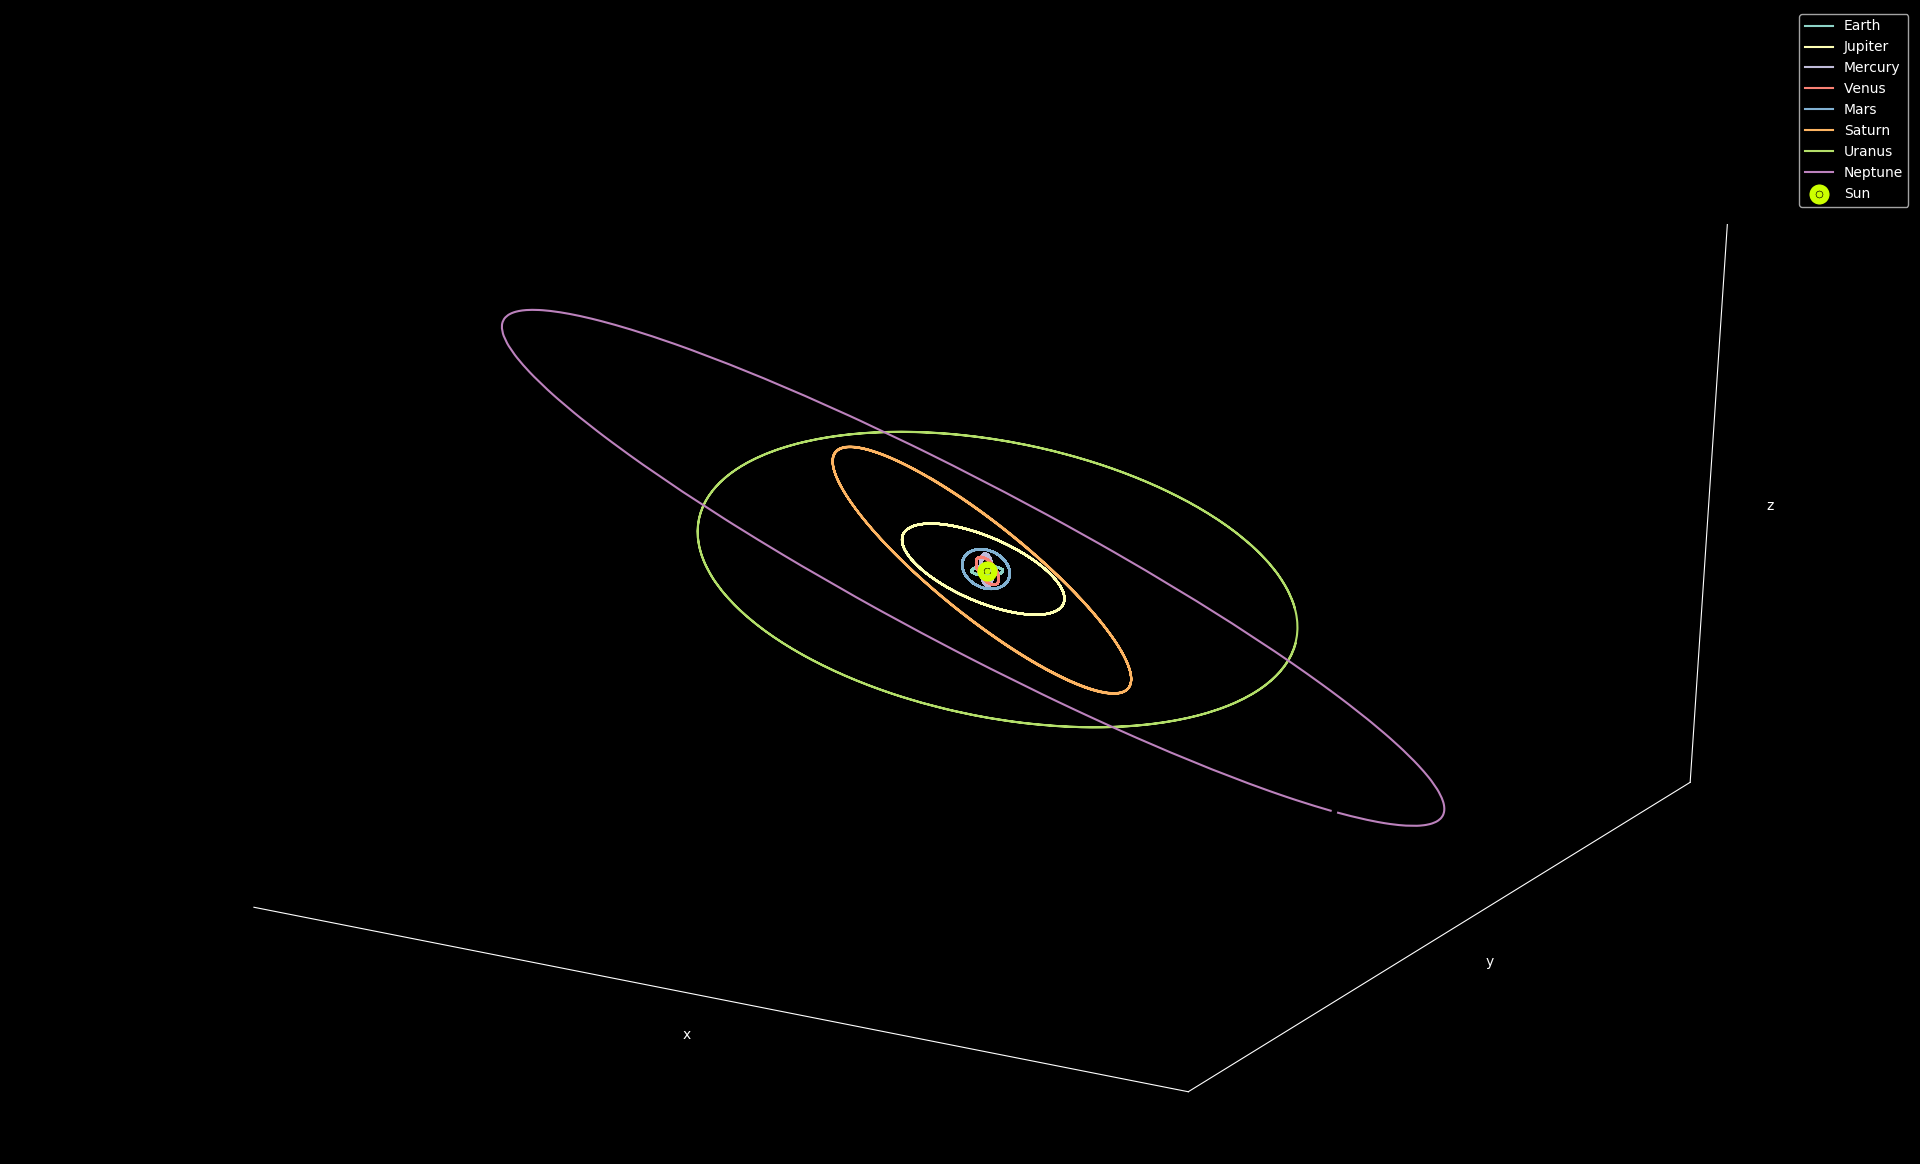
\includegraphics[width=1.2\textwidth]{./Plot/Solar_System.png}
                    \caption{: Plot of the solar system.}
                    \label{fig:solar}
                \end{center}
            \end{figure}

            From our results, when testing the program, we see that if we don't fix the position of the sun, and give it the initial velocity it has according to the NASA initial values, the Sun moves toward the center of origin. In Figure \ref{fig:solar} we have fixed the Sun, as explained in the Programming section, with very similar results, with no visible differences in the plots.

        \subsection{Perihelion of Mercury}
            The speed of Mercury at perihelion is 12.44 AU/yr, and the distance to the Sun at perihelion is 0.3075 AU. With the realtivistic constant from Equation \ref{eq:perihelion}, we get the results shown in Table \ref{tab:perihelion}.

            \begin{table}[h!]
                \caption{: $\theta_p$ of Mercury when the distance is 0.3075 AU}
                \label{tab:perihelion}
                \centering
                \begin{tabular}{l c c}

                          & Numerical angle & Real angle\\
                    \hline
                    Relativistic    & 0.02524 & 0.01194 \\
                    Newtonian   & 0.01426  &  0 \\
                    \hline
                \end{tabular}
            \end{table}

\section{Discussion}
    We have seen that the velocity Verlet method is more efficient for solving the coupled differential equations. The plot of the Earth's x and y position relative to the Sun follows respectively a cosine and a sinus curve which shows that the Earth moves in a circular orbit around the Sun.

    We also see from our results that the kinetic and potential energy, as well as the angular momentum, is conserved. These properties is conserved because if they were not conserved, the Earth would not be in orbit around the Sun.

    We saw from our numerical results that the inital velocity of the Earth needed to have a circular orbit around the Sun needs to be 2$\pi$. We can also see this analytically with the acceleration in the circular motion equal to $v^2/r$.

    \begin{flalign*}
        \frac{mv^2}r &= \frac{GM_{\odot}M_E}{r^2}\\
        v^2 &= \frac{GM_{\odot}}r\\
        v &= \sqrt{\frac{4\pi^2}1} = 2\pi
    \end{flalign*}

    Our simulations show that the inital escape velocity of the Earth was between 2.82$\pi$ and 2.83$\pi$ AU/yr. This numerical value is quite accurate compared to the exact value. We can calculate this escape velocity exact by considering the work needed to move a planet over a small distance $dr$ against the attractive force the planet feels. This work is given by:

    \begin{flalign*}
        dW &= F_G dr = -\frac{GM_{\odot}M_E}{r^2}\\
        W &= \int_r_0^\infty - G\frac{M_{\odot}M_E}{r^2} = -G \frac{M_{\odot}M_E}{r_0}
    \end{flalign*}

    This gives the minimal kinetic energy to be able to reach infinity, therefore the escape velocity $v_0$ satisfies:

    \begin{flalign*}
        W + K &= 0 \rightarrow \frac{1}2 M_Ev_0^2 = G\frac{M_{\odot}M_}{r_0}\\
        v_0 &= \sqrt{\frac{2GM_{\odot}}{r_0}} = \sqrt{2\cdot4\pi^2} AU/yr = 2.828\pi AU/yr
    \end{flalign*}

    So we see that the difference in our estimated escape velocity and the analytical one is very small. From these results we observe that if the Earth would have a higher velocity around the Sun than it does, we would be travelling away from the Sun, and we don't think that would have been appreciated here on the Earth.\\

    Further we examined how a change in the gravitational force would affect the Earth orbit around the Sun. We saw that when $\beta$ in Equation \ref{eq:beta} approches 3, the Earth starts to escape the Sun. This would have been the case if the gravitational force worked differently, so we are lucky that the gravitational force keeps us in orbit around the Sun.\\

    When we added Jupiter to the system and examined what would happen if we increased Jupiter's mass, we see that it will affect the Earth's orbit becuse the Earth will be attracted to Jupiter. When the mass is inreased by a factor of 950, we saw that the system would be stable only up to around 20 years. We can see from the plot that the Earth starts to escape the system after 20 years. When we increase the mass with a factor of 1000, we see that the Earth will immediatley escape the system, while Jupiter will stay in its orbit around the Sun.\\

    When we simulate all the planets in the Solar system, we use the initial values from NASA, which should give very accurate inital values. Our model shows that the Earth still goes in a circular orbit around the Sun. Aditionally, we can see that the orbit of Neptun is almost completed over a 164 year period, which coincides a lot with the known orbit time of Neptune. This indicates that our model gives a good representation of the real solar system.\\

    %Can the obserevd perihelion precession of Mercury be explained by the general theory of relativity?
    When we are looking at Mercury's perihelion angle it is known that when the Newtonian calculation is used, we should expect no change in the perihelion angle as the years pass. Thus, the number that is given in the results may be the error the program makes in the numerical calculations. By subtracting this error from the perihelion angle calculated with theory of relativity we get an answer closer to the correct value ($0.02524^\circ - 0.01426^\circ = 0.01098^\circ = 39,5" $). The reason for this error can come as a result of few integration points or other losses of numerical precission. \\
    Since we also know that the perihelion angle changes, we can say that the general theory of relativity is the theory that explains the perihelion precession for Mercury.

\section{Conclusion}
    In this project we have studied how the force of gravity affects objects in space, focusing on our solar system, by using both the Euler forward algorithm and the Velocity Verlet algorithm.\\ We have tweaked parameters in the force of gravity to study how the Earth moves accordingly, and adjusted the mass of Jupiter to study the movement of the Earth as well. Through this, we have obtained data on the stability of our solar system. We have also checked that our simulator program is actually able to correctly simulate our solar system, by testing it with all eight planets and the Sun in our solar system, which yielded probable results.\\
    Finally, we studied precession of Mercury according to the Sun, which gave us an idea of the loss of numerical precision we had in our program, by simulating the effect of general relativity in the gravitational force.

\newpage
\section{Bibliography}
    \href{https://github.com/emmernme/MENA-Compfys/tree/master/Project5/}{Link to our GitHub repository}\\
    \href{https://github.com/emmernme/MENA-Compfys/tree/master/Project5/OO-program/}{Link to the Object Oriented program}\\
    \href{https://github.com/emmernme/MENA-Compfys/tree/master/Project5/raw_data/}{Link to some of our raw data}\\
    \noindent \href{http://compphysics.github.io/ComputationalPhysics/doc/pub/ode/pdf/ode-print.pdf}{Lecture Slides on Differential Equations, Hjorth-Jensen Morten}\\
    \noindent \href{https://en.wikipedia.org/wiki/Escape_velocity}{Escape velocity from Wikipedia}\\

\section{Technical instructions}
    The programs we have used to calculate the various systems and test cases in this project have instructions in the top of the file explaining how to compile and run the programs. The relevant plotting programs also have these instructions.
\end{document}
